\documentclass[12pt,a4paper]{book}
\usepackage{amsmath,amsfonts,amssymb}   %% AMS mathematics macros
\usepackage{cancel} % cancel terms
\usepackage{chemfig}
\usepackage{graphicx}
\usepackage{gensymb}
\usepackage[version=4]{mhchem}
\usepackage{polyglossia}
\usepackage{fontspec}
\usepackage{titlesec}
\usepackage{lettrine}
\usepackage{xcolor}
% table with newline in headings
\usepackage{longtable}
\usepackage{makecell}
\renewcommand{\cellalign}{tl}
\renewcommand{\theadalign}{tl}
% table with newline in headings
\usepackage{epigraph, varwidth}
\usepackage{siunitx}
\renewcommand{\epigraphsize}{\small}
\setlength{\epigraphwidth}{0.9\textwidth}
% sectioning used with \paragraph{at subsubsubsection}
\setcounter{secnumdepth}{4}
\titleformat{\paragraph}
{\normalfont\normalsize\bfseries}{\theparagraph}{1em}{}
\titlespacing*{\paragraph}
{0pt}{3.25ex plus 1ex minus .2ex}{1.5ex plus .2ex}
% sectioning
\setdefaultlanguage{english}
%\setmainfont[Language=English]{Gentium Book Basic}
\setmainfont[Language=English,Scale=0.90]{IBM Plex Serif}
\setotherlanguages{marathi}
\newfontfamily\marathifont[Mapping=velthuis-sanskrit,Script=Devanagari,Language=Marathi]{Shobhika}
\usepackage{soul}
% four packages brushingupscience
\usepackage{mathpazo}
\usepackage{helvet}
\usepackage{microtype}
\usepackage[margin=15pt,font=small,labelfont={bf,sf}]{caption}
\usepackage{sectsty}
\allsectionsfont{\sffamily}
% four packages brushingupscience
% table with newline in headings
\usepackage{longtable}
\usepackage{makecell}
\renewcommand{\cellalign}{tl}
\renewcommand{\theadalign}{tl}
% table with newline in headings
\usepackage{hyperref}
\hypersetup{
    colorlinks=true,
    filecolor=magenta,
    linkcolor=blue,
    urlcolor=violet,
    citecolor=blue,
}
\urlstyle{same}
% new commands
\newcommand{\ctext}[3]{
    \colorbox{#2}{\parbox{0.9\textwidth}{\textcolor{#1}{#3}}}
}
\newcommand\TODO[1]{\colorbox{orange}{\underline{\tiny{TODO: #1}}}}
% \vect and \uvec for vector and unit vector respectively (bold)
\newcommand{\vect}[1]{\pmb{\vec{#1}}}
\newcommand{\uvec}[1]{\pmb{\hat{#1}}}
% \vect and \uvec for vector and unit vector respectively (bold)
% new commands
% other settings
\setlength{\parindent}{0pt}% Remove paragraph indent
\usepackage[skip=\medskipamount]{parskip}
% other settings
\newcommand\Problem[1]{%
   \leavevmode\par
   \stepcounter{problem}
   \noindent
   Problem \textbf{\theproblem} -- #1 \par}
\newcounter{problem}[chapter] % a new counter 'problem', resets for each ch
\newcommand\Solution[1]{%
   \stepcounter{solution}
    \leavevmode\par\noindent
   {\leftskip37pt
    Solution \textbf{\thesolution} -- #1\par}}
\newcounter{solution}[chapter] % a new counter 'solution', resets for each ch

\begin{document}
\tableofcontents
\title{Self-study Notes, Problems, and Solutions from A. P. French's Newtonian Mechanics}
\author{Kedar Mhaswade}
\date{March 2021}
\maketitle
\def\dev{\edef~{\string~}\textmarathi}

\textbf{Welcome}

These notes are from my self-study session based on A. P. French's Newtonian Mechanics \cite{apf}. There are two main objectives of these notes. The first is to study from a principal resource of interest this essential part of physics and the second is to be able to teach it to interested and driven students of mechanics. I call this a principal resource because textbooks are notoriously difficult to pick and one has got to settle with something because it is through a combination of \emph{pure reflection}, hard work, reasonable experimentation, and following of good books that a decent understanding of anything in science may be achieved. I scoured the web, consulted the venerable Physics Forums \cite{pf} and other resources and settled with \cite{apf} \emph{in the hope that French's style will resonate with me}. Of course, from time to time, I have referred to other resources where appropriate. The second objective is due, in part, to Richard Feynman who believed that teaching is a solid way to learn. Fortunately, I have access to at least one driven and talented student eager to discuss these things with me and there is some time before my engagement with him on physics starts. So, since even stalwarts like Donald Knuth require thorough preparation, I must prepare well before discussing anything on this topic with anyone. What follows is the summary of my preparation. Of course, these notes are \emph{not} to be thought of as a license to teach, rather just a prerequisite. I am keeping this in the public domain in the naive hope that someone knowledgeable reviews it at least partially and that it may prove beneficial to someone.

These notes are typeset in \LaTeX{} with the main font set to IBM Plex Serif.

In keeping with Halmos's advice \cite{iaam}: 
\epigraph{
    ``Audience, level, and treatment—a description of such matters is what prefaces are supposed to be about.''
}  

, I believe an interested high-school student with understanding of algebra, some geometry and calculus should be able to follow this material with some struggle. This is not a monograph written by me per se, but rather a collection of ideas and treatises gathered from elsewhere and written in my own words. I believe the treatment is more elementary than advanced. Finally, the focus is on solving the problems thoroughly. In solving problems, I have not referred to anything else, presumably of similar nature (e.g. ``Solutions to problems from \dots''). As an additional help, the book provides brief answers to problems. Thus, these notes are written for a personal benefit (in some abstract sense) and only incidentally for a probable benefit to someone else.

Regarding the format of \emph{notes}, I am trying something new. I am going to enumerate items in each section. This style is reminiscent of that of the books written in the $18$\textsuperscript{th} and $19$\textsuperscript{th} centuries. It may not always make the text more readable, but since the nature of this text is a review, it might be helpful. An attempt is made to solve problems serially and naturally; liberty is taken to skip some. Figures are used where appropriate.

\chapter*{Prologue}

\begin{enumerate}
    \item The book is divided into three main themes:
        \begin{enumerate}
            \item Newton's \emph{approach} to dynamics or motion
            \item Classical mechanics at work (heart of the contents)
            \item Some special topics
        \end{enumerate}
    \item Changes of motion of any object are the result of \emph{forces} acting upon it. 
    \item Although dealing with it has become our second nature\footnote{Our subconscious \emph{familiarity} with using mechanics is only second to our effortless use of a natural language}, historically, \emph{motion} has been difficult to define and precisely understand. Zeno, an ancient Greek scholar, even argued that \emph{motion couldn't exist}! Florian Cajori wrote a detailed 10-article treatise on Zeno's arguments against motion \cite{cajori-zeno} that is worth referring to. See a summary of these articles at Appendix \ref{zeno}.
    \item We routinely (or sometimes through hard work) carry out complex mechanical tasks like catching a high fly ball in baseball, driving an outswinger through covers in cricket, doing the seemingly impossible, gravity-defying gymnastic feats on floor and equipment. But it is the task of classical mechanics to \emph{discover and formulate the physical principles so that they can be applied to any situation involving forces and motions of objects big and small interacting with each other over a distance}. 
    \item The greatest triumph of classical mechanics was Newton's own success at explaining the workings of our solar system. This feat was so impressive that Alexander Pope wrote:

        \epigraph{
            Nature and Nature's Laws lay hid in the night,\\
            God said, ``Let Newton be,'' and all was light.
        }
        {
            -- \textit{Alexander Pope}
        }

    This was later corrected (as it usually happens in science): 
        \epigraph{
            It did not last; the Devil, howling ``Ho,\\
            Let Einstein be!'' restored the status quo.
        } 
        {
            -- \textit{Sir John Squire}
        }

    \item We have got to look at the scientific discoveries in a historical context. Nicolaus Copernicus had proposed \cite{copernicus} a heliocentric system in 1543. Tycho Brahe, a danish nobleman\footnote{One should listen to James Kaler's lectures on astronomy to better enjoy this historical context.}, painstakingly and comprehensively documented later in the $16\textsuperscript{th}$ century the movements of celestial bodies across the night sky. His student, Johannes Kepler, after wrestling with a tonne of data, found what looked like an ounce of truth, which he formulated in terms of Kepler's Laws (based on observations and some calculations):
        \begin{enumerate}
            \item Some bodies (planets) appear to move in ellipses (and not circles) with sun at the focus.
            \item The line joining a planet and the sun sweeps out \emph{equal areas in equal periods of time}.
            \item The ratio of the square of a planet's year (period of time it takes for it to come to the exact same position in the sky) to the cube of its mean distance from sun is the same for all the planets.
        \end{enumerate}
        However, it still looked like \emph{description} and not \emph{theory\footnote{In science, we tend to use common English words precisely. We use `theory' to mean `a well-substantiated explanation of some aspect of the natural world that usually incorporates facts, laws, inferences, calculations, and hypotheses'.}}. Newton went on to formulate the \emph{inverse-square law of gravitation} and demonstrated that Kepler's Laws were an instance of his splendid theory of gravitation.
    \item Newton \emph{quantitatively} explained the following:
        \begin{enumerate}
            \item The bulging of earth and Jupiter because of their rotation.
            \item The variation of \emph{acceleration due to gravity} with the latitude\footnote{The small circle parallel to the great equatorial circle.}.
            \item The generation of tides on earth by the combined action of sun and moon.
            \item The paths of comets through the solar system.
            \item The slow but steady change in the direction of earth's axis.
        \end{enumerate}

    \item An astonishing achievement was the prediction of a planet to explain the discrepancy in the observations on another (nearby) planet! Indeed, the story of the discovery \cite{neptune} of Neptune is fascinating!
    \item Creation of any scientific theory requires an interplay between theory and experimentation, intuition, guesswork, objectivity, and imagination. It has elements of both induction and deduction. Newton's theory is a great achievement of the human intellect, however, physics was far from complete, although a few physicists felt that way toward the end of the $19\textsuperscript{th}$ century. This was ironic (for these physicists), since the first half of the $20\textsuperscript{th}$ century saw the greatest upheaval in science since Newton!
    \item It is necessary to look at Newtonian Mechanics along with the boundaries where it is applicable and understand (though experiencing those conditions is difficult\footnote{Just like how Galileo Galilei had to postulate in the $17\textsuperscript{th}$ century that \emph{in vacuum}, the gravitational acceleration of a body is independent of its mass.}) its limitations.
    \item The currently accepted sizes and speeds of particles weave a matrix of applicable theories as shown in Figure \ref{fig: size-speed}.
        \begin{figure}[h!]
            \centering
            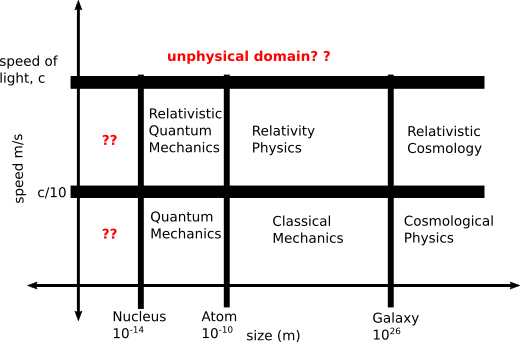
\includegraphics[width=0.5\linewidth]{size-speed.png}
            \caption{The Size, Speed, and Applicability of Physical Theories (dimensions not to scale)}
            \label{fig: size-speed}
        \end{figure}
    \item Although it is only too obvious that induction (the method of devising a general governing principle after studying only a few concrete instances) leads to error. Doing classical mechanics is more like applying inductive hypotheses that are gradually strengthened. It is not cut-and-dried like, for example, applied mathematics, where the rules are already known and one has got to apply them rigorously. With all its uncertainties, inductive hypotheses only can lead to new discoveries.
\end{enumerate}

\section{Exercises -- Hors D'ouevres}

Hors D'ouevre means ``outside work", a teaser, an appetizer. Although this section is named ``Exercises'' and not ``Problems'' (perhaps because the questions are based on what should be known beforehand and the answers could be found somewhat mechanically) there are interesting questions here.

The ``art of guessing'' \cite{polya-guessing} is emphasized in exercises. I too believe that doing a \emph{good} approximation (within 2 or 3 percent of the correct answer) rather quickly is a helpful skill that shows one's resourcefulness and understanding. One trick I often employ is to have a calculator handy, but use it only to verify the answer I have reached in my head or on paper. There are many anecdotes in this regard. This skill has generally come to be known as the ``back of the envelop calculations'' made famous by Enrico Fermi.

A recent collection of such \emph{common sense} problems in mathematics alone is available in \cite{cosm}.

It is surprising how much one can do with the help of a relatively small stock of primary data. And such data is not only of academic interest. It helps us tremendously in matters of safety in particular and living life in general. For instance, knowing that $1$ atmospheric pressure ($1$ atm) is equivalent to a 10-meter column of water and our deepest oceans are about 10-km deep, we can rather easily conclude that a marine field biologist needs to bear a pressure of 500 atm\footnote{This is \emph{enormous} pressure.} only to reach half as deep as the deepest parts of the Pacific Ocean! I agree that when life is at stake and safety paramount, detailed calculations are a must, but a quickly done \emph{reasoned estimate} often comes in handy.

\begin{longtable}{|r|l|}
\caption{Useful Bits} \label{tab: useful-bits} \\
\hline
    What & How Much \\
\hline
\endfirsthead
\endhead
    Gravitational acceleration, g & 
    $10$ \si{\metre\per\square\second} \\
 \hline
    Densities of solids and liquids & 
    $10^{3}-10^{4}$ \si{\kilogram\per\cubic\metre} \\
 \hline
    Density of air at sea level & 
    $\approx 1$ \si{\kilogram\per\cubic\metre} \\
 \hline
    Density of water at sea level & 
    $1000$ \si{\kilogram\per\cubic\metre} or $1$ g cm\textsuperscript{--3} \\
 \hline
    \makecell{Number of drops in $1$ cc ($=1$ cm\textsuperscript{--3} $=1$ ml) \\of water} & 
    $\approx25$ \\
 \hline
    Length of (Earth) day &
    $\approx 10^5$ \\
 \hline
    Length of (Earth) year &
    $\approx 31\times 10^6 \approx 10^{7.5}$ sec \\
 \hline
    Earth's radius &
    $6400$ km ($= 4000$ miles) \\
 \hline
    \makecell {Angle subtended by a finger's thickness \\
    at arm's length} &
    $\approx 1\degree$ \\
 \hline
    Thickness of paper &
    $\approx 0.1$ mm \\
 \hline
    Mass of a paperclip &
    $\approx 0.5$ g \\
 \hline
    Highest mountains, deepest oceans on earth &
    $\approx 10$ km \\
 \hline
    Earth-moon separation &
    $3.84\times 10^5$ km ($= 2.4\times 10^5$ miles) \\
 \hline
    Earth-sun separation &
    $1.5\times 10^8$ km ($= 93$ million miles) \\
 \hline
    Atmospheric pressure &
    \makecell{
        $\equiv$ to a 10-meter column of water \\
        (Use dimensional analysis to get this) \\
       $=14.7$ psi (\emph{Only in America!}) 
    } \\  
 \hline
    Avogadro's Number&
    $6.02\times10^{23}$\\
 \hline
    Atomic masses&
    $1.6\times10^{-27} - 4\times10^{-25}$\si{kg}\\
 \hline
    Linear atomic dimension&
    $\approx 10^{-10}$\si{m} $=1\si{\angstrom} $\\
 \hline
    Molecules per cc of a gas at STP &
    $2.7\times10^{19}$ \\
 \hline
    Atoms per cc in a solid &
    \makecell{$\approx 10^{23}$ (they are much more tightly packed \\
    as compared to gas!)} \\
 \hline
    Elementary charge ($e$) &
    $1.6\times 10^{-19}\si{\coulomb}$ \\
 \hline
    Electron mass &
    $\approx 10^{-30}\si{\kilo\gram}$ \\
 \hline
    Speed of light &
    $3\times 10^{8}\si{\metre\per\second}$ \\
 \hline
    Wavelengths of visible light &
    $400\si{\nano\metre}$ (violet) -- $700\si{\nano\metre}$ (red) \\
 \hline

\end{longtable}

Binomial theorem is a remarkable mathematical tool. Newton generalized it for any exponent that is a real number \cite{newton-bt} (or even a complex number):
\begin{align}
    (x+y)^{r} 
        &= \sum_{k=0}^{\infty} \binom{r}{k}x^{r-k}y^{k} \\
        &= x^r + rx^{r-1}y+\frac{r(r-1)}{2}x^{r-2}y^2+\dots \label{eqn: inf-bin-ser}
\end{align}
where $ r \in \mathbb{R}$, $k \in \mathbb{N}$, and 

$$
\binom{r}{k} 
= \frac{r\cdot(r-1)\cdot(r-2)\cdot\dots\cdot(r-k+1)}{k!}
= \frac{r^{\underline{k}}}{k!}
$$
.

Note that 
$$
r^{\underline{n}} = \prod_{k=0}^{n-1}(r-k)
$$
is called the ``$n\textsuperscript{th}$ falling factorial of $r$''.




We can use this with any \emph{real} exponent. This comes in handy in several \emph{approximations}.

When the exponent is an integer $n$, we get a finite sequence (equation (\ref{eqn: bin-theorem})) instead of the infinite series of equation (\ref{eqn: inf-bin-ser}):
\begin{equation}
    \label{eqn: bin-theorem}
(1 + x)^{n} = 1+n\cdot x + \frac{n(n-1)}{2}x^{2} +\dots + x^{n}
\end{equation}
where $n \in \mathbb{N}$. This happens because when the exponent is a positive integer, the product 
$$r
\cdot(r-1)\cdot(r-2)\dots(r-(k-1))\cdot\pmb{(r-k)}\cdot(r-(k+1))\cdot(r-(k+2))\dots
$$ 
$$
=n\cdot(n-1)\cdot(n-2)\dots(n-(k-1))\cdot\pmb{(n-k)}\cdot(n-(k+1))\cdot(n-(k+2))\dots
$$ 
must be zero for all the terms where $k > n$ (the bold term $\pmb{(r-k) = (n-k)}$ which is a part of all binomial coefficients of the terms where $k > n$ is 0).

On the other hand, when the exponent is not an integer, no binomial coefficient is zero and we get an infinite series. This \emph{dual} nature of binomial expansion is intriguing!

This leads to the approximations
\begin{equation}
\label{eqn: approx1+nx}
    (1+x)^{n} \approx 1 + nx 
\end{equation}
and
\begin{equation}
\label{eqn: approxroot1-x}
    \sqrt{1-x} = (1-x)^{\frac{1}{2}} \approx{(1+x)^{-\frac{1}{2}}} \approx 1 - \frac{1}{2}x 
\end{equation}
when $\pmb{x \ll 1}$.

For a right triangle with sides $a, b$, and hypotenuse $c$, we get
$$
    c = (a^2 + b^2)^{\frac{1}{2}} = a(1+\frac{b^2}{a^2})^{\frac{1}{2}}
$$
which leads to
\begin{equation}
\label{eqn: hypotenuse}
    c \approx a(1+\frac{b^2}{2a^{2}})
\end{equation}
when $\pmb{\frac{b}{a} \ll 1}$.

\begin{longtable}{|r|l|}
\caption{Useful Mathematical Approximations} \label{tab: useful-math-approx} \\
\hline
    What & How Much \\
\hline
\endfirsthead
\endhead
    $\pi^{2}$ &
    $\approx 10$ \\
 \hline
    $e$ &
    $\approx 2.71$ \\
 \hline
    $log_{10}e$ &
    \makecell {
        $\approx 0.43$ \\
        ($log_{e}10 \approx 2.3$)
    }\\
 \hline
    $log_{10}\pi$ &
    $\approx 0.5$ \\
 \hline
    $log_{10}2$& 
    $\approx 0.301$\\
 \hline
    $log_{10}3$& 
    $\approx 0.48$\\
 \hline
    $log_{10}5$& 
    $\approx 0.7$\\
 \hline
    $log_{10}7$& 
    $\approx 0.85$\\
 \hline
    $\pi$\si{\radian}& 
    $180\deg$\\
 \hline
    $1$\si{\radian}& 
    $\approx 57\deg$\\
 \hline
    \makecell{
        $\sin \theta$ \\
        where $\pmb{\theta \lll 1\si{\radian}}$
    } &
    $\approx \theta$\\
 \hline 
    \makecell{
        $\cos \theta$ \\
        where $\pmb{\theta \lll 1\si{\radian}}$
    } &
    $\approx 1$\\
 \hline
    $e^{x}$ & 
    \makecell {
        $=1 + x + \frac{x^2}{2!} + \frac{x^3}{3!}+\dots$\\
        $\approx 1 + x$ $\forall x \lll 1$ \\
        and then it follows that $log_e (1+x) = x $ $\forall x \lll 1$
    }\\
  \hline 
\end{longtable}

Estimation problems can be best solved with a pencil on paper\footnote{Of course, some geniuses like Von Neumann can do it in their heads.}. I have attempted to \emph{show my work} on paper whenever possible. The \emph{finished} solution, neatly typeset in \LaTeX{}, hardly shows the struggle that a paper shows. I have believed that the \emph{rough work} is more enjoyable than the \emph{fair, presentation material} although the latter might be more easily understood by others\footnote{In other words, although I like typesetting documents in \LaTeX{}, I believe that \emph{content} teaches more than the \emph{form}.}.

\Problem {
}
\Solution {
}
\Problem {
}
\Solution {
}
\Problem {
    Make reasoned estimates of
    \begin{enumerate}
        \item the total number of ancestors you would have (ignoring inbreeding) since the beginning of the human race, and
        \item the number of hairs on your head.
    \end{enumerate}
}
\Solution {
    \begin{enumerate}
        \item Population is a fascinating topic. I drew two pictures on paper that may explain my approach. Starting with ``me'' in the current generation, I drew an \emph{isolated} family tree of my family. If I now add a second isolated family (say, of my friend), then its family tree would be more-or-less identical to mine. This will proliferate the number of the \emph{First Gen} ancestors! We need to fix the number of the First Gen ancestors to some number\footnote{In Indian culture, some sages created families that cross-bred; who created those sages is left to speculation.} (I chose 2); the family trees have got to merge into each other. 
        \begin{figure}[h!]
            \centering
            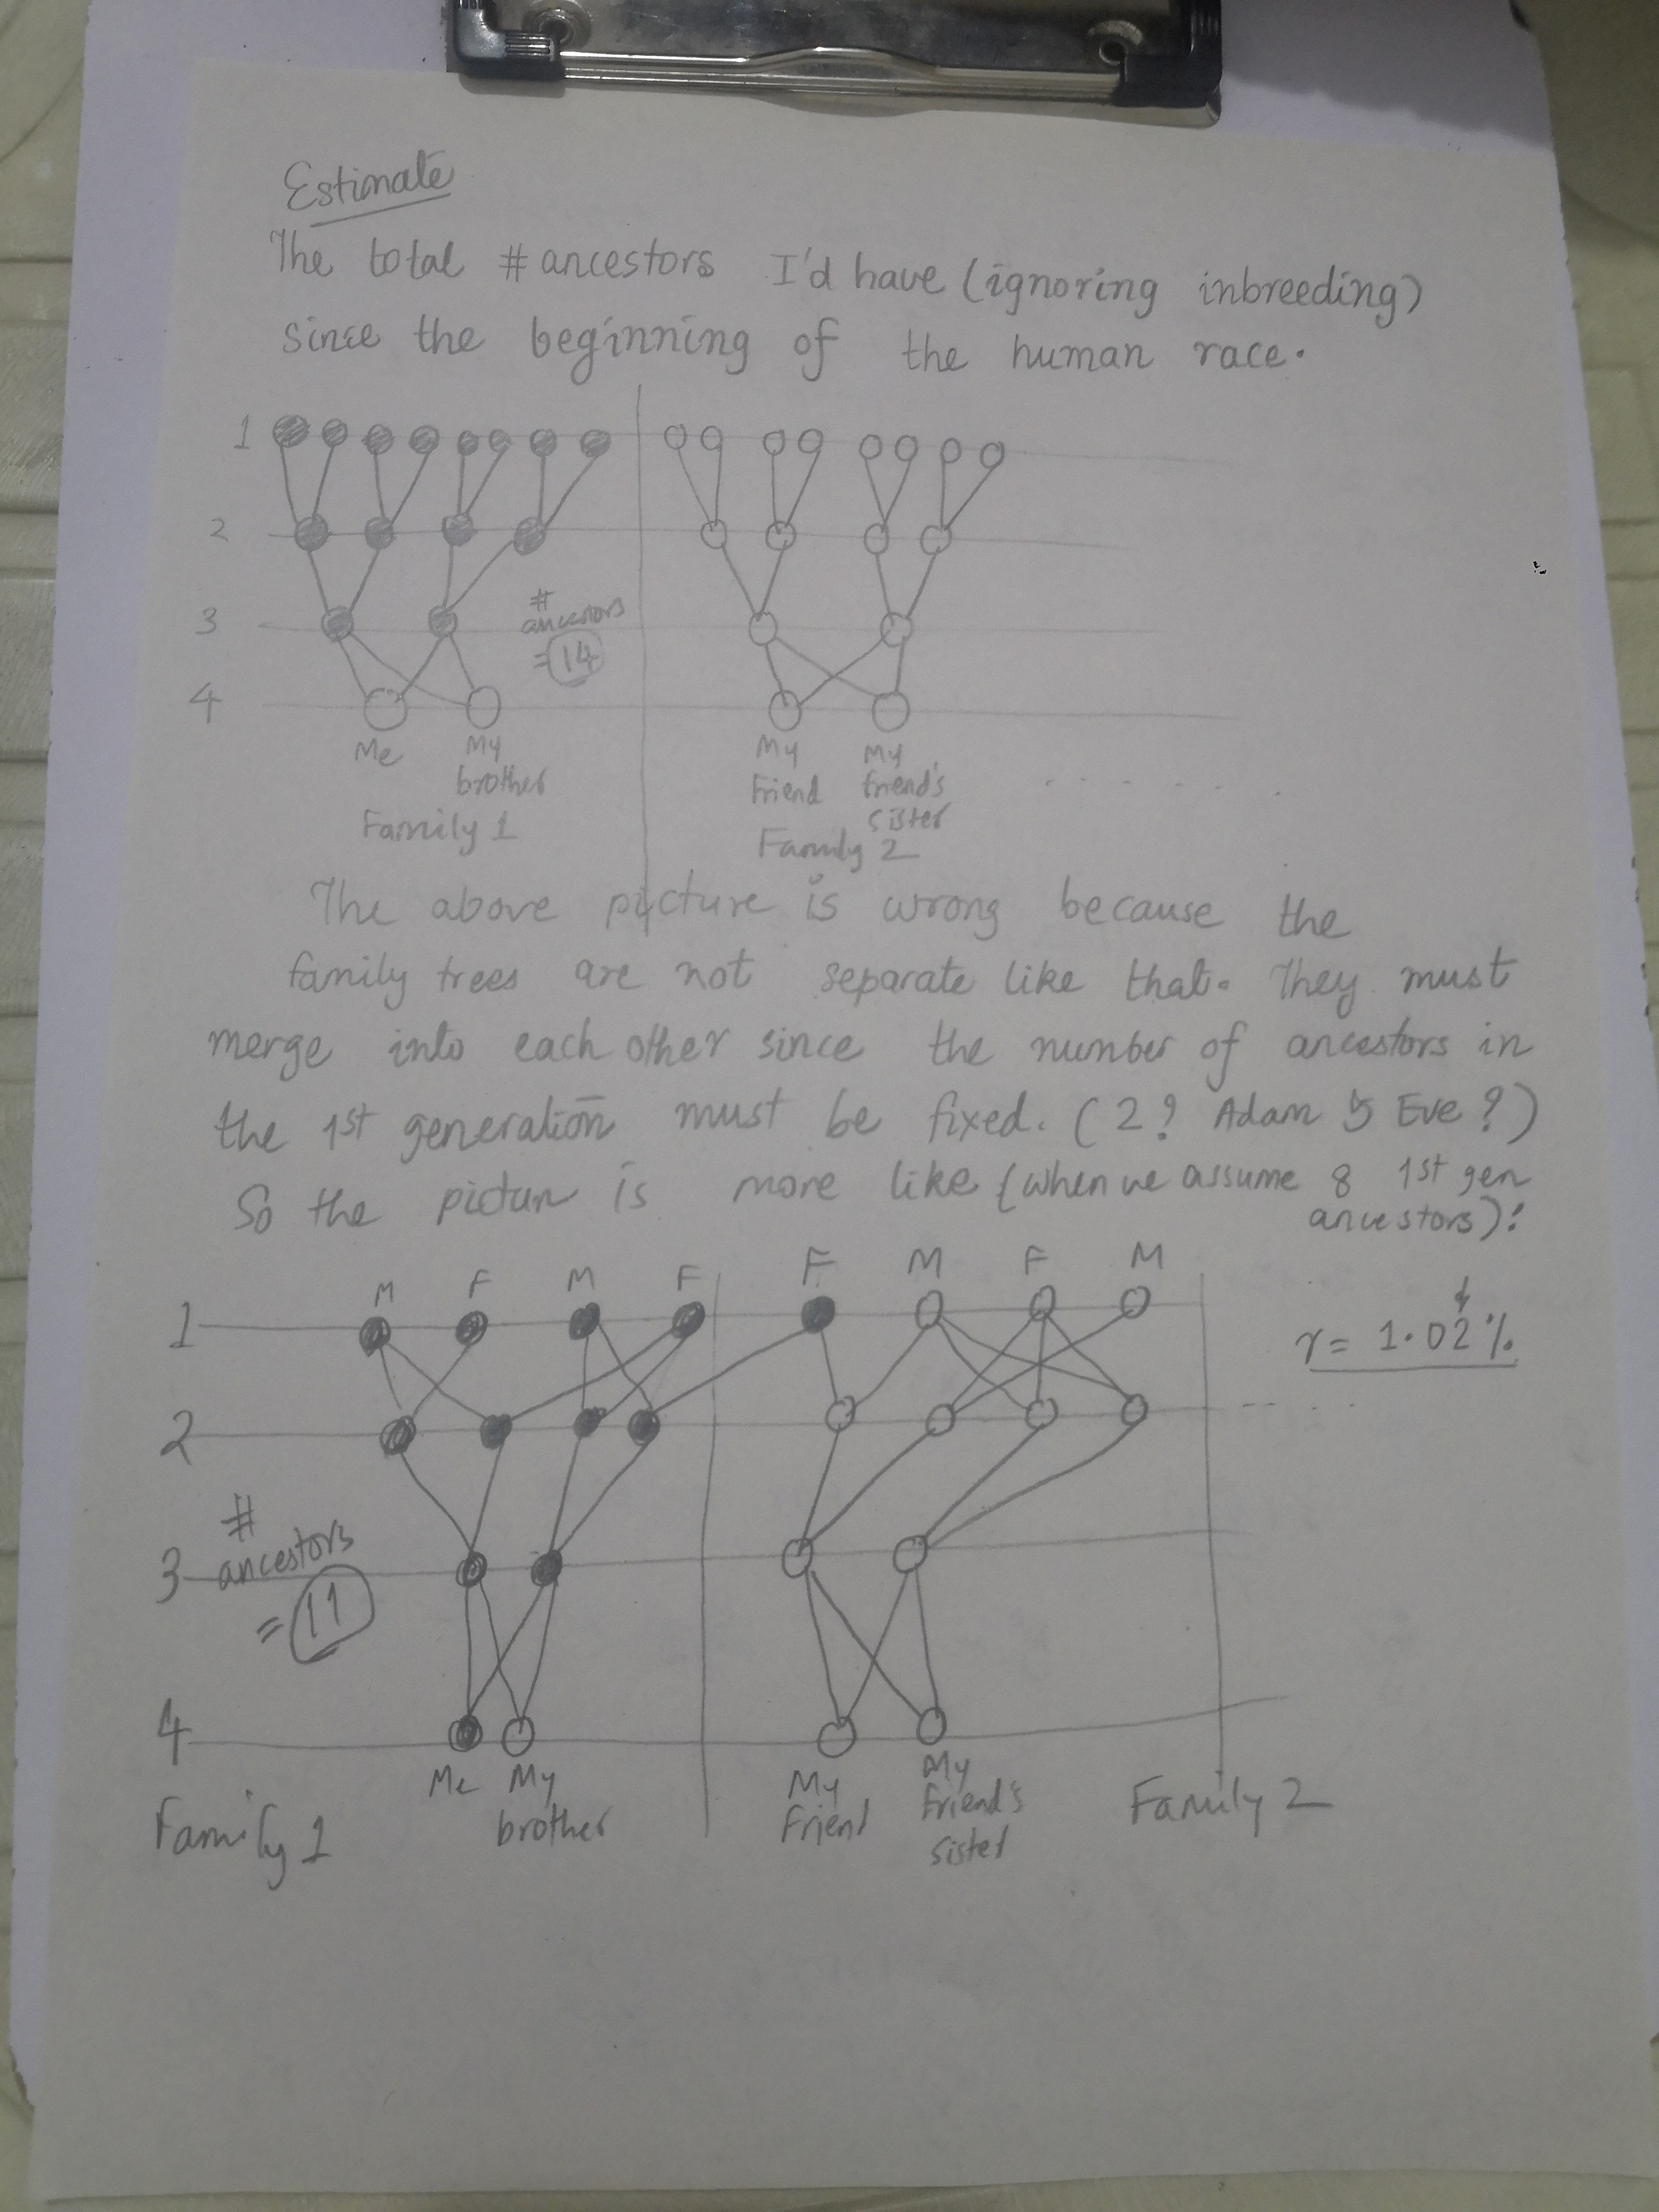
\includegraphics[width=4cm,height=5cm]{ancestry-1.jpg}
            \caption{Estimate Ancestors: 1}
            \label{fig: estimate-ancestors-1}
        \end{figure}
        \begin{figure}[h!]
            \centering
            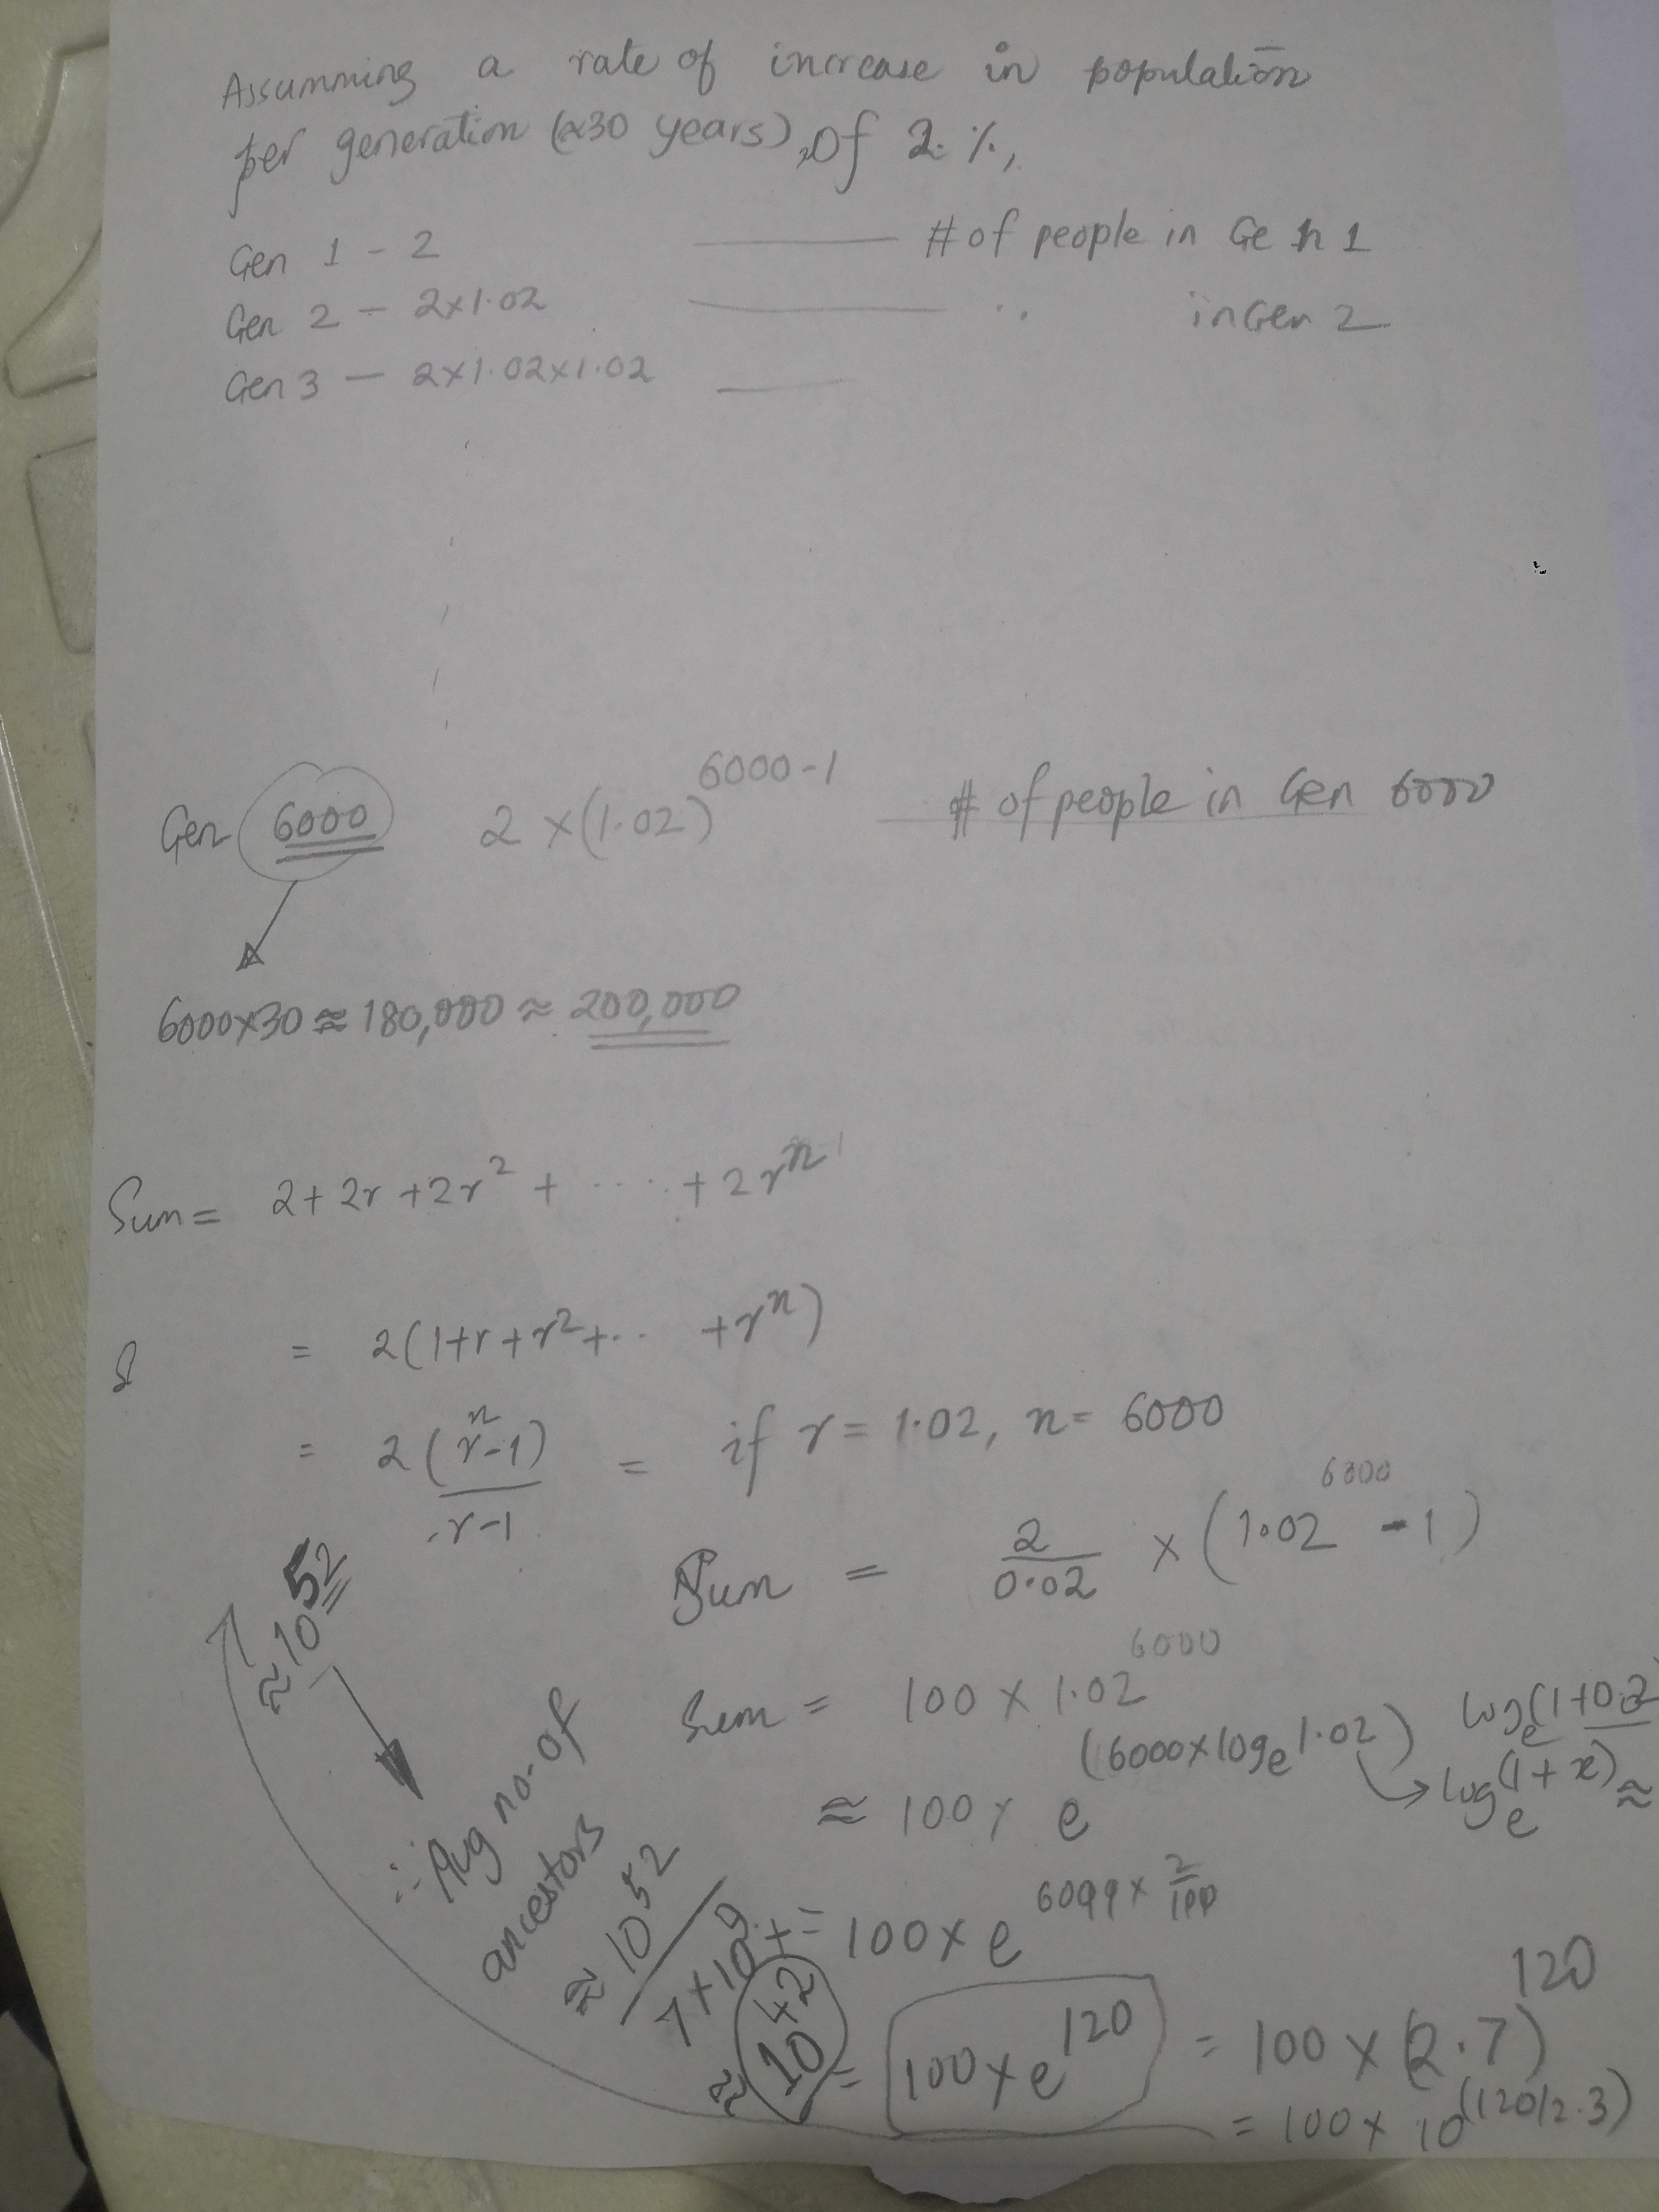
\includegraphics[width=4cm,height=5cm]{ancestry-2.jpg}
            \caption{Estimate Ancestors: 2}
            \label{fig: estimate-ancestors-2}
        \end{figure}

            When I now think of these pictures, I believe they are wrong. But documenting this process is useful. Here are some simplifying assumptions that I am now making:
            \begin{enumerate}
                \item There were 2 First Gen ancestors.
                \item On average, a generation is $25$ years. Given that human race started about $200000$ years ago, we have had about $8000$ human generations.
                \item The population of the current ($8000\textsuperscript{th}$) generation is $7\times10^9$. Due to Thomas Robert Malthus \cite{malthus}, we assume that population grows in geometric progression.
                \item \label{one-more-gen-assumption} After they give birth to their last offspring, parents live for $25$ years, i.e. one more generation.
                \item Total population up to and including the $n\textsuperscript{th}$ generation are the ancestors of the entire population of the $(n+1)\textsuperscript{th}$ generation as a whole. Therefore, if we calculate the total number of humans who ever lived up to the previous generation and divide it by some number derived from the population of the current generation alone (we must exclude the population of the previous generation from that of the current generation (see \ref{one-more-gen-assumption})), we can get the average number of ancestors of each member of the current generation.
            \end{enumerate}

            Think of first four generations. \emph{Assume} that the populations in those generations are $2$, $8$, $30$, and $90$ respectively. Then, the $2$ people in the first generation have no human ancestors, $8-2=6$ people in the second generation together have $2$ ancestors, $30-8=22$ people in the third generation together have $2+8=10$ ancestors, and $90-30=60$ people in the fourth generation together have $2+8+30=40$ ancestors.

            I hope that this simplified model appears reasonable. Let's do some calculations:
            
            Let 

            $P_n$ be the population of the $n\textsuperscript{th}$ generation; we assume $P_{8001} = 7\times 10^9$, 
            
            $r$ be the effective rate of per-generation increase of the population in a geometric progression, 
            
            $C_n$ be the cumulative population up to and including (i.e. the total number of humans who ever lived on earth) the $n\textsuperscript{th}$ generation, 
            
            $A_n$ be the number of immediate ancestors (parents) of the $n\textsuperscript{th}$ generation who are still alive. $A_{n} = P_{n-1}$,
            
            $M$ be the cumulative number of \emph{my} ancetors (I live in the $8001\textsuperscript{st}$ generation),

            $n = 8000$.

            We want to find $M$. Based on the above, for a geometric series,
            $$
                a = 2, P_{8001} = 7\times 10^{9}
            $$ 
            $$
                7\times 10^{9} = 2\cdot r^{8000}
            $$
            \begin{equation}
                \label{eqn: value-of-r}
                \therefore r = 1.0027525 
            \end{equation}
            \begin{align*}
                M 
                &= \frac{C_{8000}}{P_{8001}-A_{8001}} \\
                &= \frac{C_{8000}}{P_{8001}-P_{8000}} \\
                &= \frac{\frac{\cancel{a}\cdot(r^{7999})}{r-1}}{\cancel{a}\cdot (r^{8001}-r^{8000})} \\
                &= \frac{1}{r\cdot(r-1)^{2}} \\
                &\approx 131630 
            \end{align*}
        \item We assume that a human head has a surface area, $S$, of $100\si{\square\cm}$, only about $60\%$ of which has hair and the average radius, $r$, of a human hair is about $40\si{\micro\metre}$ giving a cross-sectional area of $\pi r^2\approx 5000\si{\square\micro\metre}$. We also assume that two hairs are about 9 hair diameters apart. The number of hairs on a human head, then, is about $120,000$:
            $$
                H = \frac{1}{10}\cdot\frac{60}{5000\times 10^{-8}}\frac{\si{\square\cm}}{\si{\square\cm}}
                  = 12\times 10^{4} 
                  = 120000
            $$
    \end{enumerate}
}
\Problem {
}
\Solution {
}
\Problem {
}
\Solution {
}
\Problem {
}
\Solution {
}
\Problem {
}
\Solution {
}
\Problem {
}
\Solution {
}
\Problem {
}
\Solution {
}
\Problem {
}
\Solution {
}
\Problem {
}
\Solution {
}
\Problem {
}
\Solution {
}
\Problem {
}
\Solution {
}
\Problem {
}
\Solution {
}
\Problem {
}
\Solution {
}
\Problem {
}
\Solution {
}
\Problem {
}
\Solution {
}
\Problem {
}
\Solution {
}
\Problem {
}
\Solution {
}
\Problem {
}
\Solution {
}
\Problem {
    How many inches per mile does a terrestrial (i.e. related to earth, land) great circle (e.g. a meridian or longitude) deviate from a straight line? 
}
\Solution {
   A sphere and its great circle share their centers and a diameter.
    \begin{figure}[h!]
        \centering
        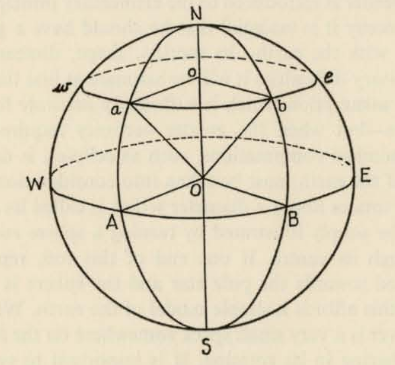
\includegraphics[width=0.5\linewidth]{sphere-great-small-circles.png}
        \caption{The terrestrial sphere. See \cite{davidson}. N-a-A-S-N, N-b-B-S-N, W-A-B-E-W are all great circles and w-a-b-e-w is a small circle. The great circles with diameter $NS$ make \emph{meridians (longitudes)} whereas the circles with diameter parallel to $WE$ make \emph{parallels (lattitudes)}. }
        \label{fig: great-small-circles}
    \end{figure}

    In the Figure \ref{fig: meridian}, as we start walking at B, if earth were flat, we would reach C after walking a mile. But since earth isn't flat, we would reach D. Thus, the deviation from the straight line $= CD$. From equation \ref{eqn: hypotenuse} we have:

    $$
    c = r(1+\frac{1}{2r^2})^{\frac{1}{2}}
    $$
    $$
    CD = c - r = r(1 + \frac{1^2}{2r^2})-r = \frac{1}{2r} = \frac{1}{8000}\text{{}mile}
    $$
    $$
    CD \approx 0.66\text{feet}
    $$
    \begin{figure}[h!]
        \centering
        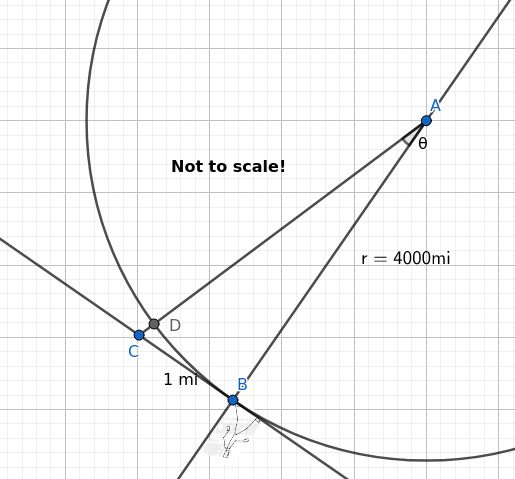
\includegraphics[width=0.4\linewidth]{meridian.png}
        \caption{Walking on the Meridian.}
        \label{fig: meridian}
    \end{figure}

}
\Problem {
}
\Solution {
}
\Problem {
}
\Solution {
}
\Problem {
}
\Solution {
}
\Problem {
}
\Solution {
}
\Problem {
}
\Solution {
}
\Problem {
}
\Solution {
}
\Problem {
}
\Solution {
}
\Problem {
}
\Solution {
}
\Problem {
    The table \ref{tab: solar-system-distances} lists the mean orbit radii of successive planets expressed in terms of the earth's orbit radius. 
\begin{longtable}{|r|l|l|l|}
\caption{Solar System Distances} \label{tab: solar-system-distances} \\
\hline
    n & Planet & $\frac{r}{r_E}$ & $log_{10}\frac{r}{r_E}$\\
\hline
\endfirsthead
\endhead
    $1$ & 
    Mercury &
    $0.39$ &
    $\approx 0.6015-1 \approx -0.4$ \\
 \hline
    $2$ & 
    Venus &
    $0.72$ &
    \makecell {
        $
        \approx log_{10}72 - 2 \approx 3*log_{10}2 + 2*log_{10}3 - 2
        $\\
        $
        \approx 3*0.3010 + 2*0.48 - 2
        $\\
        $
        \approx -0.13
        $
    }
    \\
 \hline
    $3$ & 
    Earth &
    $1$ &
    $0$ 
    \\
 \hline
    $4$ & 
    Mars &
    $1.52$ &
    \makecell {
    $
    \approx log_{10}19 + log_{10} 8 - 2
    $\\
    $
    \approx 1.28 + 0.903 - 2
    $\\
    $
    \approx 0.183
    $
    }
    \\
 \hline
    $5$ & 
    Jupiter &
    $5.2$ &
    $0.72$ 
    \\
 \hline
    $6$ & 
    Saturn &
    $9.54$ &
    $0.98$ 
    \\
 \hline
    $7$ & 
    Uranus &
    $19.2$ &
    $1.28$ 
    \\
 \hline
\end{longtable}
}
\Solution {
    \begin{enumerate}
        \item Make a graph in which $log\frac{r}{r_E}$ is ordinate (Y-coordinate) and the number $n$ abscissa (X-coordinate). On the same graph, replot the points for Jupiter, Saturn, and Uranus at values of $n$ increased by unity each. A straight line can be fitted reasonably well through the new set of points.
            \textbf{Solution}: I made this \href{https://www.desmos.com/calculator/zhewyutbx2}{plot} (Figure \ref{fig: solar-system}) using the amazing tool, Desmos \cite{desmos}.
        \begin{figure}[h!]
            \centering
            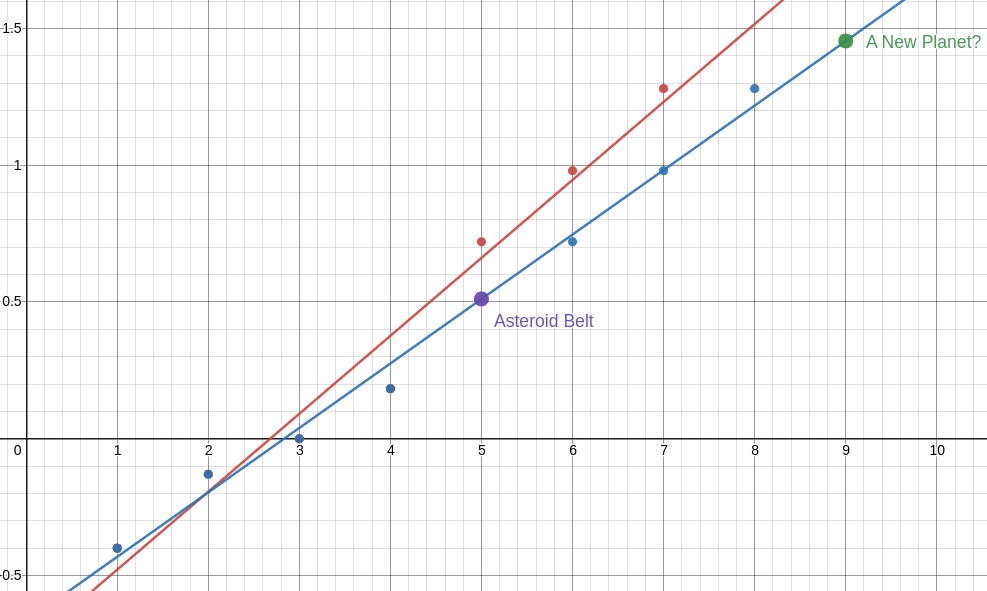
\includegraphics[width=0.6\linewidth]{solar-system.png}
            \caption{Semi-logarithmic Plot of Planet Numbers Versus Their Distances from the Sun}
            \label{fig: solar-system}
        \end{figure}
        
    \item \label{item: b} If $n=5$ in the revised plot is taken to represent the asteroid belt between the orbits of Mars and Jupiter, what value of $log \frac{r}{r_E}$ would your new graph imply for this? Compare with the actual mean radius of the asteroid belt.
        
        \textbf{Solution}: The point on the revised semi-log scale plot is $(5, 0.511)$ for the later discovered asteroid belt. This gives $\frac{r}{r_E} = 10^{0.51}=3.2$. \emph{Universe Today} \cite{universe-today} reports this to be a little less ($2.2-3.2$ AU). It appears that the mass distributed in the asteroid belt was necessary to reason about the planetary motions.

    \item \label{item: c} If $n=9$ is taken to suggest an orbit for the next planet beyond Uranus, what value would your graph imply? Compare it with observed value.

        \textbf{Solution}: The point is $(9, 1.454)$ which gives $10^{1.454}=28.44$ AU for Neptune. Britannica \cite{Neptune-data} suggests a value of $30.05$ AU. Our estimation is within an acceptable $5.66\%$ of theirs.

    \item Consider whether, in the light of (\ref{item: b}) and (\ref{item: c}), your graph can be regarded as the expression of a physical law with predictive value. (As a matter of history, it \emph{was} so used. See the account of the discovery of Neptune near the end of Chapter 8.) 

        \textbf{Solution}: The graph gives a glimpse of how the mass \emph{might have} gotten distributed into various planets, if we believe the Big Bang. The distribution then gives rise to forces of attraction due to gravity and affects the periods of planets' revolutions around the sun. The line $log \frac{r}{r_E} = 0.255\times n - 0.764$ (we found the slope and y-intercept of the line) shows some character of a physical law because it is a descriptive generalization of the planetary motion. If a planet is known to exist, then it can predict where it might be placed in the solar system.
    \end{enumerate}
}


\pagebreak

    \part{ The Approach to Newtonian Dynamics }

\epigraph
{
    It seems probable to me, that God in the beginning form'd \\
    Matter in solid, massy, hard, impenetrable, movable \\
    Particles \dots
}
{
    -- Newton, Opticks(1730)
}


\pagebreak

\chapter{A Universe of Particles} \label{ch: 2-particles}
\begin{enumerate}
    \item The \emph{essence} of the Newtonian mechanics is that the motion of a given object is analyzed in terms of the \emph{forces} to which it is subjected by its environment. 
    \item ``Particles" are difficult to define. For the purpose of Newtonian Mechanics, however, we define a particle as an object that can be treated as a \emph{point mass}.
    \item A non-exhaustive list of \emph{properties} of such particles consists of things like mass, size, shape, structure, magnetism, electric charge, and interaction with (similar or dissimilar) other particles.
    \item We ask a question: ``What is the smallest number of properties that suffices to characterize a particle?" The answer to it depends on whether the particle is \emph{elementary}. 
        \begin{enumerate}
            \item For an elementary particle, like an electron or proton, it appears that it is enough to specify its \emph{charge} and \emph{mass}. 
            \item Since larger objects which are made of many atoms are usually electrically neutral, it is enough to know their masses. Forces occur in larger objects as a result of \emph{interactions} among them and therefore, we need to know the rules of these interactions as well. Size of an object is also useful mainly because it is the magnitude of its size that helps us determine if an object can be treated as a point mass.
        \end{enumerate} 
    \item We survey particles of interest starting with smallest and go up to some of the largest known.
    \item We use SI units in this book.
    \item \textbf{In keeping with the spirit of science, things change all the time. The book has a certain (the then current) view of \emph{particles}. Particles, especially elementary particles, are researched aggressively. The 2006-view (35 years after this book was published) that is accessible to general public is captured in \cite{oerter}, and, of course, in Wikipedia's page on ``The Standard Model'' \cite{the-standard-model}.} 
    \item Electrons and Nucleons: 
        \begin{enumerate}
            \item The concept of size is not unambiguously defined for \emph{any} object.
            \item Electrons with a mass of about $9.1\times 10^{-31}\si{\kg}$ are not yet analyzed as a collection of smaller particles and hence they are fundamental particles.
            \item If we regard electron as a \emph{sphere of electric charge}, its radius is estimated to be $10^{-15}\si{m}$.
            \item Nucleons, the inhabitants of the nucleus, have a mass of about $10^{-27}\si{\kg}$. The two principle nucleons are protons (charged) and neutrons (neutral). A free proton is stable whereas a free neutron decays, in less than 15 minutes, into a proton, an electron, and an antineutrino. 
            \item Nucleons have a more complicated internal structure as compared to electrons.
        \end{enumerate}
    \item Atomic Nuclei:
        \begin{enumerate}
            \item The smallest and lightest nucleus is of course one proton (which is the same as a hydrogen \emph{ion} (\ce{H+})). 
            \item The heaviest naturally occurring nucleus (that of \ce{U^{238}_{92}}) contains 238 nucleons. (\textbf{Before introducing a uranium nucleus, perhaps we should mention that there are 92 different, naturally occurring nuclei (along with electrons), each of which has a characteristic number of nucleons. This is a miracle in itself. Each such nucleus is that of an \emph{element}.})
            \item If we assume that nucleons are equally densely packed in each element's nucleus, we get (denoting the nuclear mass by $m$ and spherical nuclear volume by $v$):
                $$
                    \frac{m_1}{v_1} = \frac{m_2}{v_2}
                $$
                $$
                    \frac{m_n\times A_1}{\frac{4}{3}\pi r_1^{3}}
                    =
                    \frac{m_n\times A_2}{\frac{4}{3}\pi r_2^{3}}
                $$
                where $m_n$ denotes the mass of \emph{a} nucleon (which is the same for each element), $A$ the atomic mass number (that is a fancy name for the number of nucleons) of an element.

                Upon simplification, we can see ($\frac{r_1^3}{r_2^3}=\frac{A_1}{A_2}$) that the diameter of a nucleus is roughly proportional to the cube root of its atomic mass number, $A$.
            \item \label{item: density-of-nucleus} The unit of distance, \emph{Fermi, F} (named after the Italian physicist Enrico Fermi), is used to denote the extremely small nuclear distances: $1 F = 10^{-15}\si{\m}$. This can give us some sense of how dense nuclear material is, although it is difficult to comprehend such a dense matter:
                $$
                    d_U = \frac{4\times 10^{-25}}{\frac{4}{3}\pi (10\times 10^{-15})^3} \approx 10^{17}\si{\kg\per\cubic\metre} 
                $$
                That makes the uranium nucleus $100$ trillion times as dense as water.
        \end{enumerate}
    \item Atoms:
        \begin{enumerate}
            \item Chemists had established for elements a \emph{relative mass scale} giving hydrogen a mass of $1$. The idea of \emph{mole} was introduced as \textbf{that amount of a pure substance whose mass in grams is numerically equal to its relative mass on this scale.}
            \item Avogadro's brilliant idea (of course, others contributed to it as well) of a \emph{mole} (\si{\mol}) said that equal moles of a pure substance (an element or compound) must contain equal numbers of their fundamental particles (atoms or molecules). Thus, $1\si{\mol}$ of hydrogen contains as many \ce{H} atoms as the number of \ce{H2O} molecules in $1\si{\mol}$ of water or sucrose molecules in $1\si{\mol}$ of sucrose. Although it was known that $2\si{\mol}$ of hydrogen combine with $1\si{\mol}$ of oxygen to produce $1\si{\mol}$ water, the number of molecules or atoms in a mole (the so-called Avogadro's constant) itself was unknown.
            \item Existence of the \emph{characteristic mass transfers} in electrolysis of ionic compounds (e.g. \ce{NaCl, ZnCl2, AgCl}) suggested a strong link between charge and atomic mass. Based on the amount of an ionic substance collected under a known electric potential at the electrodes, a correlation could be established. After precise measurement of electric charge by Millikan's experiments, atomic masses were established.
            \item The mass-to-charge ratio is measured by mass spectroscopy today.
            \item An \emph{atomic mass unit, amu,} is defined as $\frac{1}{12}$ of the mass of the isotope \ce{^{12}C} (carbon $12$).

                $1 \text{amu} = 1.67\times 10^{-27}\si{\kg}$
            \item Mass of an atom is roughly the same as the mass of its nucleus, but its diameter is about $10^4$ times of that of the nucleus.
            \item The diameter of an atom is expressed in \si{\angstrom}:
                $1\si{\angstrom} = 10^{-10}\si{\m} = 10^5 F$.
            \item The heaviest atoms are \emph{not} markedly bigger than the lightest ones. The general trend in the periodic table is that the atomic radius increases down a group and decreases across a period to the right. Alkali metals have the highest atomic radii in a given period.        
            \item The atoms or molecules of a gas at normal atmospheric pressure are separated from one another, on average, by about 10 times their diameter. 
        \end{enumerate}
    \item Molecules and Living Cells:
        \begin{enumerate}
            \item A convenient unit to represent sizes of things that are of interest to biologists is \emph{micron}. $1 \text{ micron}=10^{-6}\si{\m}$. 
            \item On average, a human cell is about $10\text{ micron}$ in diameter. Then, the estimated number of cells (assuming we have as many cells as there is non cellular matter) in a human body of volume $0.1\si{\cubic\metre}$ is 
                $$
                    n_c = \frac{0.1}{2\times\frac{4}{3}\pi\times125\times10^{-18}}
                    \approx 10^{14}
                $$
                
                A $70\si{\kg}$ human who has about $10^{14}$ cells has, on average, a cell mass, 
                $$
                    m_c = \frac{70}{10^{14}}\si{\kg} = 7\times10^{-13}\si{\kg}
                $$

                Human body comprises $65\% \ce{O}$, $18.5\% \ce{C}$, $9\% \ce{H}$, $3.2\% \ce{N}$, and $1\% \ce{P}$ \emph{by mass}. Then, on average, an atom of the human body has a mass of:
                $$
                    m_a = 0.65\times 8 + 0.185\times 12 + 0.09 + 0.032\times 7 + 0.01\times 15 \text{ amu}
                $$
                $$
                    m_a \approx 7.9 \text{ amu} \approx 13.19\times10^{-27}\si{\kg}
                $$

                Thus the number of atoms in a human cell on average = $\frac{m_c}{m_a} = 0.5\times10^{14}$.
        \end{enumerate}
    \item Sand and Dust:
        \begin{enumerate}
            \item These particles, predominantly of quartz (crystalline \ce{SiO2}) are chemically inert. 
            \item The earth's surface is loaded with such particles (humans build houses that need sand as well). 
            \item Windblown particles have a diameter of about $0.01\si{\mm}-1\si{\mm}$. Below that size the material is airborne. Smallest dust particles are about $0.1 \text{ micron}$ in diameter. 
        \end{enumerate}
    \item Other Terrestrial (Belonging to Earth) Objects: These include objects in the range of masses $10\si{\mg}-1000\si{\kg}$.
    \item Planets and Satellites:
        \begin{enumerate}
            \item It does not occur to us to treat Earth as a particle while we are on it, but once we are able to leave it to go into the Space, we can think of it as a tiny speck.
            \item Planets in the solar system can be regarded as point masses because of the vastness of the empty space. Of course, we need to take into account little distances and masses if the problem (e.g. tides on Earth) requires us to do so.
            \item Mercury is the smallest planet and Jupiter is the largest. Earth is the densest. Together the planets \textbf{represent almost all of the mass around the sun in our solar system; Jupiter alone represents almost $\frac{2}{3}$}.
            \item Planets have natural (and to a very small extent artificial) satellites. Examples of interesting artificial satellites (space probes) are the Hubble telescope, the International Space Station, Cassini that, while orbiting Saturn, crashed into Saturn (by design) after its mission was complete. In addition to these satellites, we have a belt of tens of thousands of tiny asteroids\footnote{For professional astronomers, these, along with some wealthy humans' artificial satellites being planned to be sent into the Space 2020-30, are the \emph{vermin of the skies}.}  between Mars and Jupiter that orbit the Sun.
        \end{enumerate}
    \item Stars:
        \begin{enumerate}
            \item Stars are the most gigantic chemical plants we know. There is just so much going on on a star! And yet, when, with a naked eye, we look at it in the night sky and all it does is illuminate brightly or twinkle making us disbelieve any and all of the facts like, ``Our Sun has space for \textbf{$1$ million} Earths and that it is losing $4$ million metric tonnes a second."
            \item Astronomical distances are so large that a convenient unit of distance is 1 light-year which is the distance light travels in vacuum in a year = $9.46\times10^{15}\si{\m}$. The nearest star the sun is about 4 light-years which is roughly $25$ trillion = $25000000000000$ miles away. Even when stars are massive, the interstellar separation is even more astounding. The ratio of diameters of large stars to the separation distance is of the order of $10^{-7}$ or $10^{-8}$.  It is very difficult to achieve the kind of vacuum that exists in the Space in a laboratory. 
            \item Even though stars are huge, the interstellar distances allow us to use them as particles.
        \end{enumerate}
    \item Galaxies:
        \begin{enumerate}
            \item By 1924, Edwin Hubble produced a conclusive proof that our own Galaxy (which was mistaken, before 1920's, for the universe) was only one of innumerable systems of the same general kind. 
            \item Galaxies are clusters of stars.
                \epigraph
                {
                    Galaxies are the largest single aggregates of stars in the universe. They are to astronomy what atoms are to physics. 
                }
                {
                    --\textit{Adam Sandage}
                }
            \item A galaxy can contain anywhere between $10^{6}-10^{11}$ stars!
            \item And yet, the intergalactic distances make galaxies themselves as particles!
            \item Since galaxies are receding from each other at a speed proportional to the intergalactic distances\footnote{Another of Hubble's astounding findings.}, it may so happen that -- because of ``galactic red shift'', the energy from them falls short of reaching us -- a limit is put on the knowable universe.
            \item If we assume the density of matter throughout the Space as $10^{-26}\si{\kg\per\cubic\m}$ and volume of the order of $(10^{26})^3$, then the total mass is about $10^{52}\si{\kg}$ which will correspond to about $10^{11}$ galaxies.
            \item These masses and distances, that is, a \emph{particulate} view of the matter is a strong candidate for the application of Newtonian mechanics.
        \end{enumerate}
\end{enumerate}
\Problem {
}
\Solution {
}
\Problem {
}
\Solution {
}
\Problem {
    Calculate the approximate mass, in tons, of a teaspoonful of nuclear matter.
}
\Solution {

    $1$ tsp = $4.92\si{\ml}$.

    We have already established (see \ref{item: density-of-nucleus}) that nuclear matter is about $10^{14}$ times as dense as water. Therefore the mass of nuclear matter that only occupies 1 teaspoon, 

    $$
      m = 4.92\times10^{14}\si{\g}
    $$
    $$
      m = 4.92\times10^{14}\si{\g} = 4.92\times10^{8}\si{\tonne}
    $$
    $$
        m\approx 500\text{ million tonne}
    $$
    (The book says it is $10^9\si{\tonne}$ which is off by a factor of 2.)
}

\Problem {
    Sir James Jeans once suggested that each time any one of us draws a breath, there is a good chance that this lungful of air contains at least one molecule from the last breath of Julius Caesar. Make your own calculation to test this hypothesis.
}
\Solution {
    The volume of air in a breath, the so-called tidal volume, is estimated to be about $500\si{\ml} = 500\si{\cubic\cm}$. Assuming an air of density $1.2\si{\kg\per\cubic\metre}$, the \emph{amount} of air in a human breath = $1.2\times 500\times 10^{-6}\si{\kg} = 6\times10^{-4}\si{\kg} = 0.6\si{\g}$. Assuming the molar mass of air to be $29\si{\g}$, 
    $$
        n_b = \frac{0.6\times6.022\times10^{23}}{29}\approx 1.23\times10^{22}
    $$
    where, $n_b$ is the number of \emph{molecules} in a human breath. When Julius Caesar breathed his last, he exhaled $n_b$ molecules into the atmosphere.

    Atmosphere of Earth is extremely complex. Its mass is estimated to be about $5.1\times10^{18}\si{\kg} = 5.1\times10^{21}\si{\g}$.
    $$
        n_a = \frac{5.1\times10^{21}\times6.022\times10^{23}}{29}\approx10^{44}
    $$
    where $n_a$ is the approximate number of molecules in the atmosphere.
    We can now see that \emph{the fraction} of atmosphere that was Caesar's last breath was: 
    $$
    \frac{n_b}{n_a} = \frac{1.23\times10^{22}}{10^{44}}
    \approx 1.23\times10^{-22}
    $$
    which is slightly higher than $\frac{1}{n_b}=0.8\times10^{-22}$ the fraction of my breath that $1$ molecule represents.

    It appears that Sir James Jeans knew very well what he was talking about.
}

\chapter{Space, Time, and Motion} \label{ch: 3-space-time-motion}
\epigraph
{
    Hitherto I have laid down the definitions of such words as are less known, and explained the sense in which I would have them to be understood in the following discourse. I do not define time, space, place, and motion, since they are well known to all. Only I must observe, that the vulgar (i.e. the common people) conceive those quantities under no other notions but from the relation they bear to sensible objects. And from there arise certain prejudices, for the removing of which, it will be convenient to distinguish them into absolute and relative, true and apparent, mathematical and common.
}
{
    --\textit{NEWTON, Principia (1686) \cite{principia}}
}
\begin{enumerate}
    \item What is Motion?
        \begin{enumerate}
            \item Our ability to give any precise account of motion depends upon the use of two separate concepts: \emph{space} and \emph{time}. \textbf{We say that an object is moving if it occupies different positions at different instants}.
            \item Our ideas of motion align with those of Newton himself. Again, in keeping with the changing and falsifiable nature of science, these notions that Newton himself had are inadequate in the light of what we have learned since Newton's time. Here (in a pair of square brackets) are some of Newton's assertions which appear plausible, but should be \emph{taken with a dose of healthy skepticism}:
                \begin{enumerate}
                    \item {[Space is absolute.]}
                    \item {[Absolute Space, in its own nature, without relation to anything external, remains always similar and immoveable.]}
                    \item {[Each object in the universe exists at a particular point in space and time.]}
                    \item {[Our physical measurements agree with the theorems of Euclidean geometry and Space is assumed to be Euclidean.]}
                    \item {[Time is also absolute and flows on without regard to any physical object or event. Principia \cite{principia} says, ``Absolute, true, and mathematical time, of itself, and from its own nature, flows equably without relation to anything external, and by another name is called \emph{duration}: relative, apparent, and common time is some sensible and external (whether accurate or equable\footnote{i.e. not varying}) measure of duration by means of motion, which is commonly used instead of \emph{true time} \dots'']}
                    \item {[One can neither speed up nor slow down the \emph{rate of the flow of time} and it exists uniformly throughout the universe. Identical and synchronized clocks placed anywhere in the universe can correctly mark off the flow of absolute time and remain synchronized forever.]}
                    \item {[Space and Time are, although independent, in a sense interrelated.]}
                \end{enumerate}
                It was later found that although they sound plausible, many of the above ideas have consequences that are inconsistent with experience. This first became clearer with motions at very high ($\approx c$, the speed of light) speeds. This is not to say that Newton was not aware of relativistic ideas, but that it appears that he believed in an absolute space and time. It is true that we are unable to experience absolute motion: Right now, although the tree or the table that you are looking at is moving in an absolute sense, you are not able to experience that movement; you believe that it is stationary. A. I. A. Adewole carefully went through what Newton wrote in his Principia \cite{principia} at \cite{adewole} and here is the summary of his commentary on Newton's views on \emph{Absolute Space}:
                \begin{enumerate}
                    \item Our freedom to relate motion to any designated body of our choice is \emph{not} hindered by the existence of \emph{absolute space}. In other words, some body does \emph{not} need to be at \emph{absolute rest} for us to relate motion of some other body to it. If the body we chose happens to be at absolute rest, then any motion \emph{with respect to it} will also be absolute, otherwise, it will not be absolute.
                    \item As long as we are only interested in \emph{relative motions} of bodies, we can choose any body whatsoever and only consider those motions \emph{with respect to it}.
                    \item The fact that relative motion can be with respect to any body does not disprove the existence of an absolute space.
                    \item We are unable to distinguish the ``state of rest'' from the ``state of uniform motion'' in both relative space and absolute space. 
                \end{enumerate}
        \end{enumerate}
    \item Frames of Reference:
        \begin{enumerate}
            \item ``A car is moving'' implies that ``There is a relative motion between a car and earth (and all the things like trees, buildings etc. that are firmly attached to the earth)''.
            \item We accept the \emph{local surroundings} -- a collection of objects firmly attached to earth and therefore at rest relative to each other -- as defining a \emph{frame of reference} with respect to which the changes in position of other objects can be observed and measured.
            \item The choice of a frame of reference is arbitrary, of course. However, it is convenient to choose a frame of reference in which \emph{the description of motion is simplest}. Thus, while describing the motion of a car on earth or the movement of a roller-coaster, it is convenient to use a frame of reference that is attached to the earth rather than to the sun (which has a motion relative to earth and vice versa).
        \end{enumerate}
        For an excellent video introduction to frames of reference see \cite{pssc-for}. There are theoretical reasons to choose some reference frames to others that we shall see later \TODO{ref here}.
    \item Coordinate Systems:
        \begin{enumerate}
            \item A frame of reference is defined by some array of physical objects \emph{that remain at rest relative to each other}.
            \item \emph{The Space of our experience} has three dimensions, we need to specify three independent quantities in order to uniquely fix the position of a point in Space.
            \item Problems we consider are mainly two- and three-dimensional.
            \item In a 2-D plane, we have the so-called Cartesian $(x, y)$ and Polar coordinates$(r, \theta)$ of a point P that are equivalent:
                \begin{equation}
                    \label{eqn: 2-d-coordinates}
                    \mbox{In 2-D}
                    \begin{cases}
                        r^2 = x^2 + y^2 \\
                        \tan{\theta} = \frac{y}{x} \\
                        x = r\cdot \cos{\theta} \hspace{1cm} y = r\cdot \sin{\theta}
                    \end{cases}
                \end{equation}
            \item In Cartesian coordinate system, if we denote $\uvec{i}$ and $\uvec{j}$ as \emph{unit vector}s in the $x-$ and $y-$ directions respectively, we get
                \begin{equation}
                    \label{eqn: vector-addition-cartesian}
                    \mbox{(In 2-D)}\hspace{1cm} \vect{r} = x\uvec{i} + y\uvec{j}
                \end{equation}
                where $\vect{r}$ is the \emph{position vector} of $P(x, y)$.
            \item \label{item: 2-d-polar-vector} 
                In Polar coordinate system, if $\uvec{e_r}$ is the unit vector in the direction of the radius vector $\vect{r}$ and $\uvec{e_\theta}$ the unit vector in the direction perpendicular to the radius vector, then we get $\vect{r} = r\uvec{e_r}$. Note that $\uvec{e_\theta}$ is not used in this expression, but it will be used often.
            \item For the 3-D space, the most generally useful coordinate systems are the 3-D Cartesian coordinates $(x, y, z)$ and Spherical Polar coordinates $(r, \theta, \varphi)$. 
                \begin{equation}
                    \label{eqn: 3d-vector-cartesian}
                    \vect{r} = x\uvec{i} + y\uvec{j} + z\uvec{k}
                \end{equation}
                where, like $\uvec{i}$ and $\uvec{j}$, $\uvec{k}$ is the \emph{unit vector} in the $+z$-axis.
                For a more detailed description of the Spherical Coordinate System, see \cite{polar}.
            \item We use the right-handed Cartesian system. This means that if a \emph{right-handed screw} is rotated from $+x$-axis toward $+y$-axis, it will move in the direction of $+z$-axis. Authors adopt different conventions, but we'll adopt the convention that is shown in Figure \ref{fig: spherical-polar}. According to this convention,
                \begin{enumerate}
                    \item The coordinates are $(r, \theta, \varphi)$.
                    \item The $+z$-axis is called the \emph{zenith}.
                    \item The angle $\theta$ that the position vector of $P(x, y, z)$ makes with the $z+$-axis is called the \emph{polar angle}. $0\leq\theta\leq\pi$. The complementary angle $\lambda = \frac{\pi}{2}-\theta$ is called the \emph{latitude} of $P$.
                    \item The angle $\varphi$ that the \emph{orthographic projection} of $P$ in the $XY$-plane (the so-called plane of the meridian) makes with the $+x$-axis is called the \emph{azimuthal angle}. $-\pi\leq\varphi\leq\pi$. $\varphi$ is also called the \emph{longitude} of $P$.
                \end{enumerate}
                    \begin{figure}[h!]
                        \centering
                        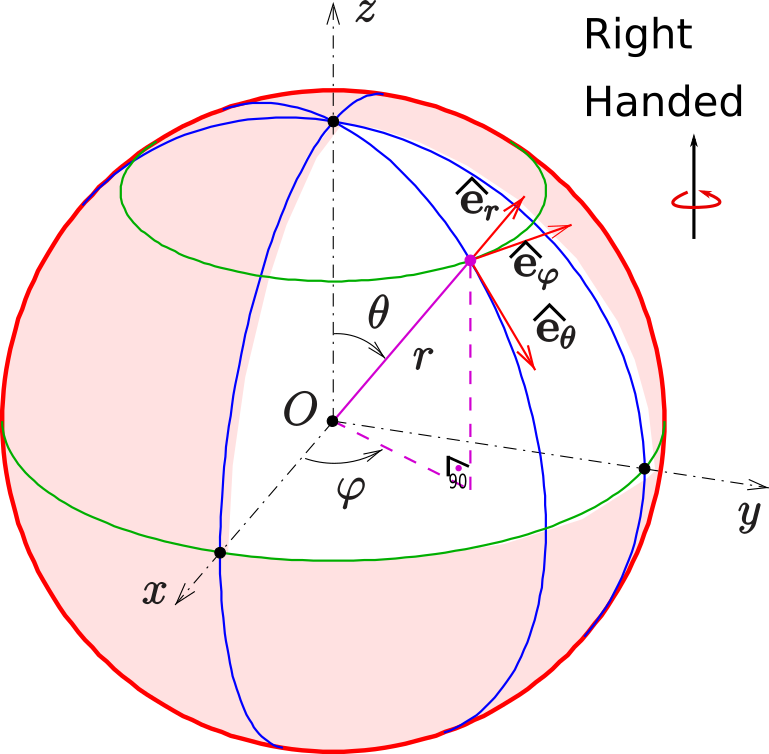
\includegraphics[width=0.5\linewidth]{Kugelkoord-lokale-Basis-s-modified.png}
                        \caption{The Spherical Polar Coordinate System}
                        \label{fig: spherical-polar}
                    \end{figure}
            \item Cartesian coordinates in terms of Spherical Polar coordinates:
                \begin{equation}
                    \label{eqn: from-polar-to-cartesian}
                    \mbox{In 3-D}
                    \begin{cases}
                        x = r\sin\theta\cos\varphi \\
                        y = r\sin\theta\sin\varphi \\
                        z = r\cos\theta
                    \end{cases}
                \end{equation}
            \item Spherical Polar coordinates in terms of Cartesian coordinates:
                \begin{equation*}
                    \label{eqn: from-cartesian-to-polar}
                    \mbox{In 3-D}
                    \begin{cases}
                        r = \sqrt{x^2+y^2+z^2} \\
                        \theta = \arccos{\frac{z}{r}} = \arccos{\frac{z}{\sqrt{x^2+y^2+z^2}}}\\
                        \varphi = \text{atan2}{\frac{y}{x}}
                    \end{cases}
                \end{equation*}
                where the function $atan2$ returns the angle in Euclidean plane, in radians, from the $+x$-axis to the ray joining $P(x,y)$ and the origin $O(0,0)$; $-\pi\leq\text{atan2}\frac{y}{x}\leq\pi$.
            \item In the vector notation for Spherical Polar coordinates, we have three unit vectors (you can imagine standing on the surface of the sphere at $P$):
                \begin{enumerate}
                    \item $\uvec{e_r}$ -- the unit vector along $OP$; this points vertically upward. As in the case of two dimensions (see: \ref{item: 2-d-polar-vector}), $\vect{r} = r\uvec{e_r}$.
                    \item $\uvec{e_\theta}$ -- the unit vector perpendicular to $OP$; this points due south.
                    \item $\uvec{e_\varphi}$ -- the unit vector also perpendicular to $OP$; this points due east.
                \end{enumerate}
        \end{enumerate}
    \item Combination of Vector Displacements: This item is really a very short sampler on vectors.
        \begin{enumerate}
            \item Vectors are directed entities with magnitude. This is not a thorough definition as not everything with a direction and magnitude is called a vector. On the other hand, certain vectors may not have both direction and magnitude.
            \item In this context, an entity that has magnitude but no direction is called a \emph{scalar}. When the term ``vector'' is \emph{not} in context, scalar just means number.
            \item Historically, vectors were defined before the formal definition of \emph{vector spaces} and vector fields (see \cite{vector-wikipedia}). Therefore, in physics, we sometimes talk of vectors without referring to vector spaces to which they belong.
            \item If an entity is defined in mathematics, interesting (and perhaps useful) things start to occur when an instance of such entity combines with another. Interesting things also happen when an instance of one entity combines with an instance of another entity. In other words, \emph{operations on entities} are perhaps more interesting than the entities in isolation. In essence, defining axioms of vector calculus is what vector spaces do. Few operations on vectors are more frequent than others (although all are useful):
                \begin{enumerate}
                    \item \emph{Adding} two vectors
                    \item \emph{Scaling} a vector, that is, growing or shrinking its magnitude by a number (or \emph{scalar})
                    \item \emph{Multiplying} two vectors
                \end{enumerate}
            \item Since the topic of vectors is developed by various mathematicians, physicists, and other scientists, there are various assumptions and interpretations. In general, in physics, the location of a vector does \emph{not} matter. As long as two vectors have the same magnitude and direction, they are equivalent, wherever in the space they are located.
        \end{enumerate}
    \item Resolution of Vectors:
        \begin{enumerate}
            \item The choice of the \emph{coordinate system} is arbitrary. Once we have decided a convenient coordinate system (it does \emph{not} matter whether the axes are orthogonal), however, we can resolve a vector into components along those axes. The \emph{vector sum} of components of a vector along the axes of all possible coordinate systems always yields the same vector.
            \item The $n-$dimensional vector space and a not-necessarily-orthogonal coordinate system are of interest from a generalization standpoint (See \cite{resolution-q-phy-fo}), but we will stick to an orthogonal coordinate system \textbf{unless stated otherwise} and illustrate it using two dimensions.
            \item The following is then given:
                \begin{figure}[h!]
                    \centering
                    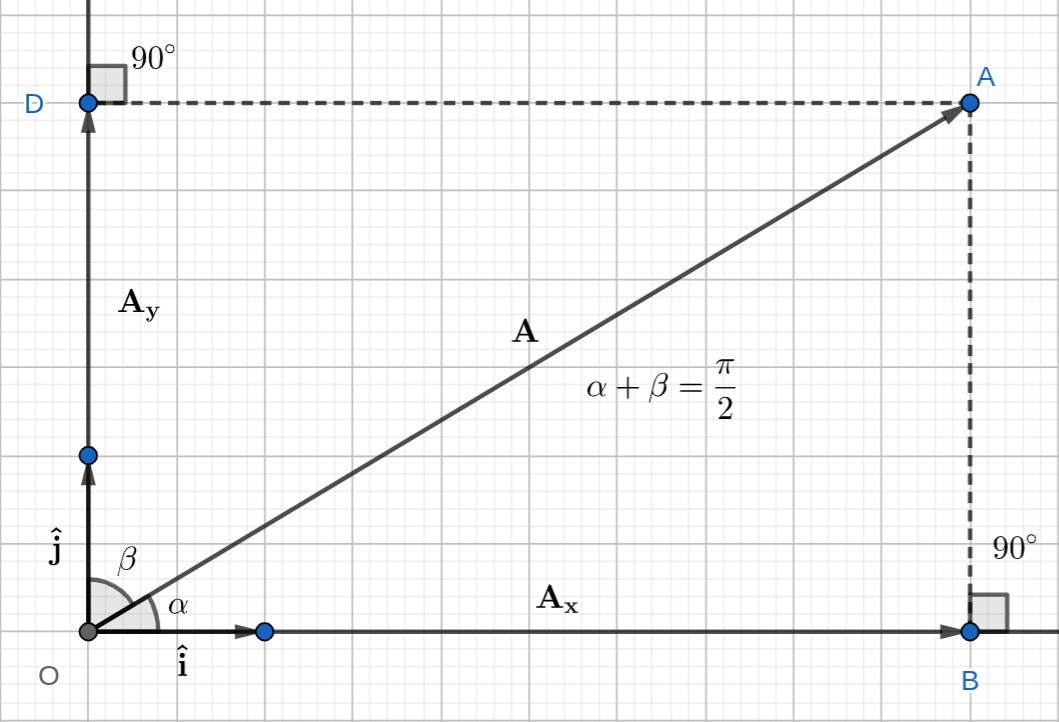
\includegraphics[width=0.7\linewidth]{basic-2d-orthogonal-axes.png}
                    \caption{Basic 2-D Orthogonal Axes}
                    \label{fig: basic-orthogonal-2d}
                \end{figure}
                \begin{enumerate}
                    \item The unit vectors (sometimes called the \emph{Basis}) are denoted $\uvec{i}, \uvec{j}, \uvec{k}$. A vector is denoted by a bold capital letter with an arrow on top: $\vect{A}, \vect{P}$. The magitudes (which are numbers, or scalars) of vectors are denoted simply by a capital letter: $A$, $B$. 
                    \item The \emph{scaling} of a vector $\vect{A}$ by a number $n, n\in\mathbb{R}$ is denoted as a vector $n\vect{A}$, which is simply a vector whose magnitude is $\lvert n\rvert$ times $A$, the magnitude of $\vect{A}$. If $n$ is negative, the scaled vector points in the exact opposite direction as $\vect{A}$, otherwise it points in the same direction as $\vect{A}$.
                    \item A vector $\vect{A}$ (in two dimensions) can be resolved as:
                        $$
                            \vect{A} = A_{x}\uvec{i}+A_{y}\uvec{j}
                                     = (A\cos\alpha)\uvec{i} + (A\cos\beta)\uvec{j}
                        $$
                    \item The \emph{scalar product} (also called the \emph{dot product}) of two vectors $\vect{A}$ and $\vect{B}$ that are at an angle $\theta$ is defined as a number:
                        $$
                        \vect{A}\cdot\vect{B} = A\cdot B\cdot\cos\theta
                        $$
                        Therefore, since $\lvert\uvec{i}\rvert = \lvert\uvec{j}\rvert = 1$, we get:
                        $$
                            A_x = \vect{A}\cdot\uvec{i}
                        $$
                        $$
                            A_y = \vect{A}\cdot\uvec{j}
                        $$
                        and
                        $$
                            \vect{A} = (\vect{A}\cdot\uvec{i})\uvec{i}+(\vect{A}\cdot\uvec{j})\uvec{j}
                        $$
                    \item The above, although rather straightforward, may feel complicated. But it is useful in \emph{relating} the components of a given vector in \emph{different coordinate systems}. Consider, for instance, a coordinate system $x^\prime y^\prime$ obtained by rotating the $xy$ coordinate system by an angle $\theta$ (See Figure \ref{fig: basic-orthogonal-2d-rotated}). Let the unit vectors in the new system be $\uvec{i^\prime}, \uvec{j^\prime}$ respectively.
                \begin{figure}[h!]
                    \centering
                    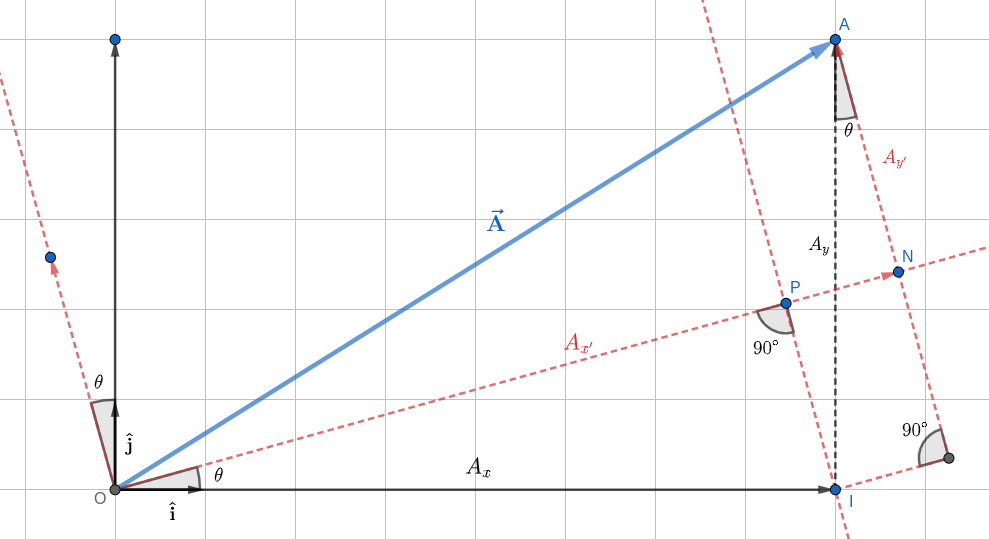
\includegraphics[width=0.8\linewidth]{basic-2d-orthogonal-axes-rotated.png}
                    \caption{Basic 2-D Orthogonal Axes (rotated from Figure \ref{fig: basic-orthogonal-2d})}
                    \label{fig: basic-orthogonal-2d-rotated}
                \end{figure}
                        $$
                            \vect{A} = A_x\uvec{i} + A_y\uvec{j} = A_{x^\prime}\uvec{i^\prime} + A_{y^\prime}\uvec{j^\prime}                        
                        $$
                        \textbf{We are interested in finding $A_{x^\prime}$, $A_{y^\prime}$ in terms of $A_x, A_y$}.
                        Taking the scalar product (which distributes over vector addition) of the above equation once with $\uvec{i^\prime}$ and once with $\uvec{j^\prime}$, we get:
                        $$
                            A_{x^\prime} = A_x(\uvec{i}\cdot\uvec{i^\prime}) + A_y(\uvec{j}\cdot\uvec{i^\prime})
                        $$
                        and
                        $$
                            A_{y^\prime} = A_x(\uvec{i}\cdot\uvec{j^\prime}) + A_y(\uvec{j}\cdot\uvec{j^\prime})
                        $$
                        because $\uvec{i}\cdot\uvec{i} = \uvec{j}\cdot\uvec{j} = \uvec{i^\prime}\cdot\uvec{i^\prime} = \uvec{j^\prime}\cdot\uvec{j^\prime} = 1$ and $\uvec{i}\cdot\uvec{j} = \uvec{i^\prime}\cdot\uvec{j^\prime} = 0$. And,
                        $$
                            A_{x^\prime} = A_x\cos\theta + A_y\sin\theta
                        $$
                        $$
                            A_{y^\prime} = -A_x\sin\theta + A_y\cos\theta
                        $$
                        because $\uvec{i}\cdot\uvec{i^\prime} = \cos\theta$, $\uvec{j}\cdot\uvec{i} = \cos(\frac{\pi}{2} + \theta) = -\sin\theta$, $\uvec{j}\cdot\uvec{i^\prime} = \cos(\frac{\pi}{2}-\theta) = \sin\theta$, and $\uvec{j}\cdot\uvec{j^\prime} = \cos\theta$.

                        The ease of algebraic manipulation (which can be generalized to more dimensions) is perhaps clear. In the Figure (\ref{fig: basic-orthogonal-2d-rotated}) one can see the geometric interpretation of the same result.

                        This can be generalized to a non-orthogonal or oblique coordinate system as well.
                        \begin{figure}[h!]
                            \centering
                            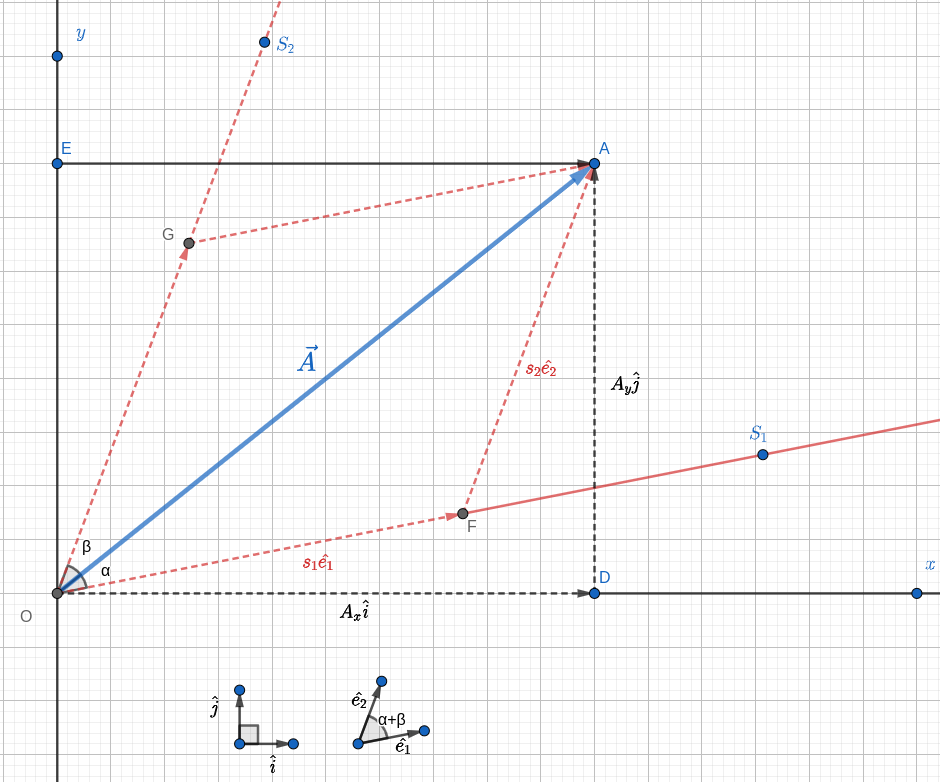
\includegraphics[width=0.8\linewidth]{oblique-2d-system.png}
                            \caption{Finding Vector Components Along Non-orthogonal Axes}
                            \label{fig: oblique-2d-system}
                        \end{figure}

                        $$
                            \vect{A} = A_x\uvec{i} + A_y\uvec{j} = s_1{\uvec{e_1}} + s_2{\uvec{e_2}}
                        $$
                        Taking the scalar product (which distributes over vector addition) of the above equation once with $\uvec{e_1}$ and once with $\uvec{e_2}$, we get:
                        $$
                            A_x(\uvec{i}\cdot\uvec{e_1}) + A_y(\uvec{j}\cdot\uvec{e_1}) 
                            =
                            s_1 + s_2(\uvec{e_2}\cdot\uvec{e_1})
                        $$
                        $$
                            A_x(\uvec{i}\cdot\uvec{e_2}) + A_y(\uvec{j}\cdot\uvec{e_2}) 
                            =
                            s_1(\uvec{e_1}\cdot\uvec{e_2}) + s_2
                        $$
                        Since the axes are not orthogonal anymore, the scalar product $\uvec{e_1}\cdot\uvec{e_2}$ does \emph{not} vanish. Nevertheless, the two above equations are linear in $s_1$, $s_2$ which can be solved since we know $A_x$, $A_y$ and can find the scalar products $\uvec{i}\cdot\uvec{e_1}$, $\uvec{i}\cdot\uvec{e_2}$, $\uvec{j}\cdot\uvec{e_1}$, $\uvec{j}\cdot\uvec{e_2}$, and $\uvec{e_1}\cdot\uvec{e_2}$ knowing the various angles like $\alpha$, $\beta$, and $\theta$ (for example, $\uvec{i}\cdot\uvec{e_1} = \cos\theta$ if the angle between the $x-$ and $S_1-$ axes is $\theta$).

                        \textbf{However, the use of oblique coordinate system like this is rather special}.
                \end{enumerate}
        \end{enumerate}
    \item Vector Addition and the Properties of Space:
        \TODO{Revisit}
        \begin{enumerate}
            \item 
        \end{enumerate}
    \item Time:
                \epigraph
                {
                    What is time? The shadow on the dial, the striking of the clock, the running of the sand, day and night, summer and winter, months, years, centuries -- these are but arbitrary and outward signs, the measure of time, not time itself \dots
                }
                {
                    --\textit{Longfellow, Hyperion, Bk. II, Ch. 6}
                }
                \epigraph
                {
                    What is time then? If nobody asks me, I know; but if I were desirous to explain it to one that should ask me, plainly, I do not know.
                }
                {
                    --\textit{St. Augustine}
                }
        \begin{enumerate}
            \item Although we \emph{think we know} what time is, defining it is very hard.
            \item Our concept of the passage of time is tied directly to the fact that things \emph{change}. Would we have \emph{felt} that the time passes had there been no perceptible change to observe?
            \item A special case of the observation or experience that the things change is that \emph{the things repeat or recur}. Such \emph{recurrent} things have been, in fact, a human experience that is more common than the experience of things that merely change. With recurrent things comes the idea of a ``time interval''. It is not easy to satisfactorily answer if the time interval between two successive occurrences of an event is the same. Here are a few examples:
                \begin{enumerate}
                    \item Sun rises in the east repeatedly. We become so accustomed to this experience that we say that the same amount of time passes between every two successive sunrises. We tend to treat the same way two successive occurrences of many other recurring events. How are we so sure that exact same amount of time passes between two sunrises?  
                    \item The human heart beats every so often. How are we sure that the heart beats are \emph{not} erratic?
                    \item Many of us celebrate birthdays and anniversaries repeatedly. How are we sure that the same amount of time has passed in between any two successive birthdays?
                \end{enumerate}
            \item  Although it may be valuable (as an intelligent construction perhaps) to have an abstract concept of time continuously flowing, our first-hand experience with time is only the observed behavior of a device called ``clock''. To find out the duration of process we simply associate the beginning and the end of the process with the readings of a clock. As \cite{nbs-time-freq} describes, in early times, the location of sun the sky was the only reliable indication of the time of the day at a place on earth. When sun was not visible, one was unable to know the time with precision. Clocks were developed to \emph{interpolate between the checks} with the sun which got the status of the \emph{master clock}. The idea of motion is intricately related to the idea of time. Thus, although it may not be a must, people used some kind of repeating motion, most notably, a \emph{pendulum} to construct clocks. The pendulum is attached to the hands on a clock face through a system of gears. The hands are moved a fixed amount on each swing of the pendulum. In effect, the gears and hands count \emph{the number of the pendulum swings} that are then converted into hours, minutes, and seconds.
            \item Unfortunately, mechanical pendulum clocks have an annoying characteristic: They \emph{lose} time or stability due to effects of, for example, friction. Therefore, we need to look for \emph{more stable ``pendulums''}. One such source of \emph{periodic} motion is the natural atomic resonance or vibrations. An atom is seen vibrating with a certain frequency of resonance. What does it really mean? It means that when an atom is placed in a radiation field of certain energy\footnote{The field should provide an energy that allows the loosely bound valence electron of the atom to \emph{jump} to outer orbits, thereby producing a resonance that is characteristic of the atom; if the energy does not match with the energy required by orbits, there is no resonance.}, it absorbs energy only in \emph{quanta} or packets of energy. The absorbed energy pushes the valence electron to a higher orbit. When the electron returns to its original orbit, the energy is emitted in the form of light of certain frequency (remember that light is an electromagnetic wave with certain frequency?). This makes an atom an excellent \emph{resonator} for clocks. 
            \item Timekeeping, time scales, astronomical time, atomic time, and related topics are of great interest. Refer to \cite{sundials-atomic} and \cite{nbs-time-freq} for engrossing accounts of the theory and fundamentals.
            \item Whether or not the ultimate abstraction of uniform flow of time has any meaning, we approach the measurement of time \emph{as if} such a flow existed. And then, when we proceed from individual measurements to general equations involving time, we introduce time as a \emph{continuous variable} $t$ in a mathematical sense.
        \end{enumerate}
    \item Units of Standards of Length and Time:

        Length:
        \begin{enumerate}
            \item Measurement is heart of science. However, measurements are prone to error. The two characteristics of measuring devices that are of essence are: accuracy and reproducibility. The accepted standards for these characteristics of measuring various fundamental physical properties like mass, length, and time evolve. 
            \item Refer to Wikipedia's definition of $1\si{\metre}$.
        \end{enumerate}
        
        Time:
        \begin{enumerate}
            \item Although comparing the measurement of a physical property of any object with that of a \emph{standard object} is fraught with issues, the nature of time poses additional challenge: one cannot \emph{store} the length of any time interval for a later use.
            \item Refer to Wikipedia's definition of $1\si{\second}$.
        \end{enumerate}

        It is believed that physical constants might change. For instance, the great physicist P. A. M. Dirac suggested that the \emph{constant} of universal gravitation might be changing, albeit very slowly.

        \epigraph
        {
            \dots This matter of units and standards is one that most of us do not bother our heads with. We \emph{think} we know what is meant by a meter or a second; and a ruler or a watch is usually near at hand. But perhaps the above discussion may help to suggest that the detailed story of how these basic measures are defined, refined, and made more and more precise is a quite fascinating business -- especially, perhaps, for time, to which astronomical observations over the centuries have contributed data of a refinement that almost passes belief (something ``passes belief'' means it is extremely difficult to believe).
        }
        {
            --\textit{A. P. French, Newtonian Mechanics, pp. 65}
        }
    \item For the current (2019) refinement and redefinition of the SI units, NIST has a series of fascinating articles. See \cite{nist-revised-si}. Every interested reader should read these articles carefully.
    \item Here is a list of recommended readings in ``measurement'':
        \begin{enumerate}
            \item PSSC Physics \cite{pssc-physics}.
            \item Physics for the Inquiring Mind \cite{pim} and Teaching Physics for the Inquiring Mind \cite{tpim}.
            \item An Introduction to the Physics of Mass, Length, and Time \cite{intro-to-phy-mass-length-time}.
            \item The Voices of Time \cite{voices-of-time}: A cooperative survey of man's views of time as expressed by the sciences and by the humanities.
            \item The Standards of Time and Frequency \cite{stf} and The Standards of Time and Frequency at the Outset of the 21st Century \cite{stf21}.
            \item The Nature of Time \cite{nature-of-time}.
            \item Time and Physical World \cite{time-and-physical-world}.
        \end{enumerate}
    \item Velocity
        \begin{enumerate}
            \item Velocity is a measure of how fast something has moved and in what direction. Since we pay attention to the direction, velocity becomes a \emph{vector}. The ideas of time, space (``displacement'' is a more frequently used term in this context), and velocity are intimately related. 
            \item Average Velocity: To measure the movement of a particle, we can measure its displacement from one point in space to another and how long it took for the particle to traverse the distance between those points in one dimension. Dividing the displacement by the time taken gives the \emph{speed} of the particle. Speed gives us only an overall idea about how fast the particle moved without any regards to the direction of movement. Velocity is directed speed. Speed is the magnitude (a scalar) of velocity.
                
                It is perhaps easier to always think of velocity \emph{not as one thing}, but as a combination of two things -- the distance covered and the time taken. Thus, to the question, ``How fast did you drive the car to the city?'', ``Reasonably fast, 100 kilometres in 2 hours'', is a more straightforward answer than ``Reasonably fast, at 50 kilometres per hour.'' (even though we routinely say it this way). Dividing the \emph{total displacement} by the \emph{total time} is akin to calculating the average value of some property of discrete items: For example, calculating the average height of a group of people by dividing the sum of their heights (which is equivalent to the total displacement) by the number of people (which is equivalent to the total time taken). A subtle difference in these two examples (speed and average height of a group of people) is in the units used to express them. Height is measured in units of length (for example, centimetres) and average height is also calculated in the same units (that is, we do \emph{not} say that the average height is $159.5$ cm per person, but that the average height \emph{of the group} is $159.5$ cm). Displacement is measured in units of length (e.g. kilometres) but the average speed is calculated in the units of length divided by units of time (e.g. kilometres \emph{per hour}). 
                This subtlety happens with the value (or magnitude) of every quantity, like speed, that is \emph{derived} from other quantities.

                There is no \emph{specific} name (like, for example, \emph{Newton} which is the name for the unit of force) for any unit of speed\footnote{There is the ``knot'' which is one nautical mile per hour.}. Typically, such name is given in the honor of the scientist who contributed a lot to our understanding of the entity that the unit \emph{specifies}. The fact that speed or velocity units don't bear such names may be surprising at first, but it only goes to show that velocity and speed have intrigued humanity for ages!

                One can rather naturally visualize such a characterization of the (average) speed by \emph{plotting} the distance covered \emph{against} the time taken. On a ``Cartesian Plane'', for example, we can plot the time taken in hours to reach somewhere on the X-axis and the distance to it in kilometres from the start on the Y-axis. Then, we will end up with two points $(0, 0)$ (specifying the start) and $(2, 100)$ (specifying the finish). That's it, we get exactly two points A and B and nothing else as in Figure \ref{fig: a-first-s-t-plot}.
                        \begin{figure}[h!]
                            \centering
                            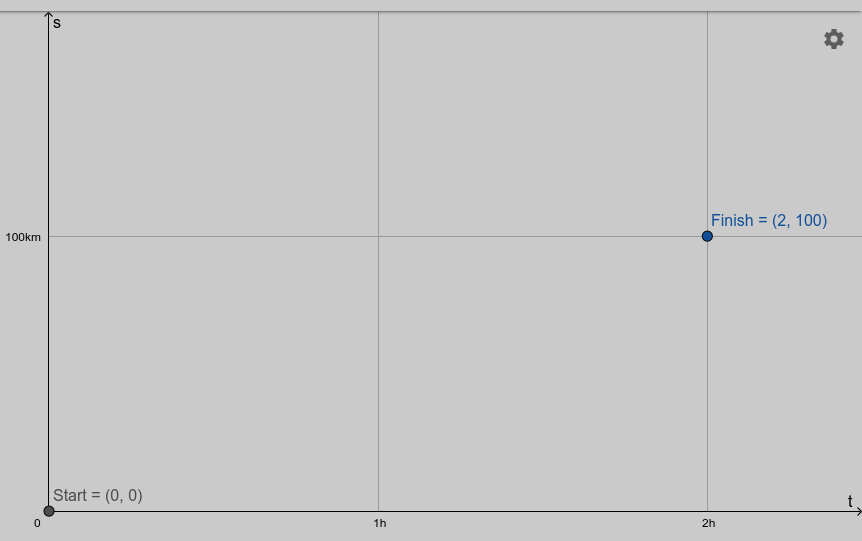
\includegraphics[width=0.5\linewidth]{a-first-s-t-plot.png}
                            \caption{A First Plot of Time Taken and Distance Covered}
                            \label{fig: a-first-s-t-plot}
                        \end{figure}

                Such a ``discrete'' plot clearly does not tell the ``whole story'' of the journey from point A to point B. Since we are plotting the distance from A on Y-axis and time taken on X-axis, we know that both the values are monotonically increasing (that is we never go ``back in time'' or ``back \emph{toward} the starting point A''). But exactly how the distance from A increases as time passes is not clear from the plot. To get an idea, imagine that we measured the distances covered at regular time intervals as we went along from point A to point B. This might give us a plot as in Figure \ref{fig: a-second-s-t-plot}.
                        \begin{figure}[h!]
                            \centering
                            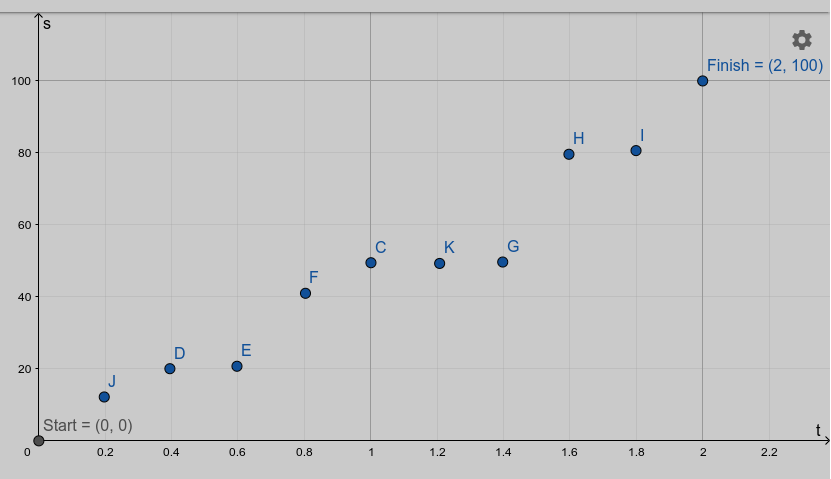
\includegraphics[width=0.5\linewidth]{a-second-s-t-plot.png}
                            \caption{A Second Plot of Time Taken and Distance Covered}
                            \label{fig: a-second-s-t-plot}
                        \end{figure}
                This helps us visualize where you were, for example, $36$ minutes or $1$ hour into the journey. If we only do more of what we just did, we can plot even more points. And, if we assume that the motion of the car was not extraordinarily erratic or jerky, we can conceive a line that shows the trend of how displacement changes with time. As far as the plot is concerned, this is our transition from the discrete to the continuous. The plot becomes a curve as shown in Figure \ref{fig: displacement-as-a-function-of-time}, and, as such, we can think of the displacement as a \emph{mathematical function} of time which assumes the role of an \emph{independent variable}. Knowing the value of time we can find the displacement of the car from its starting point.
                        \begin{figure}[h!]
                            \centering
                            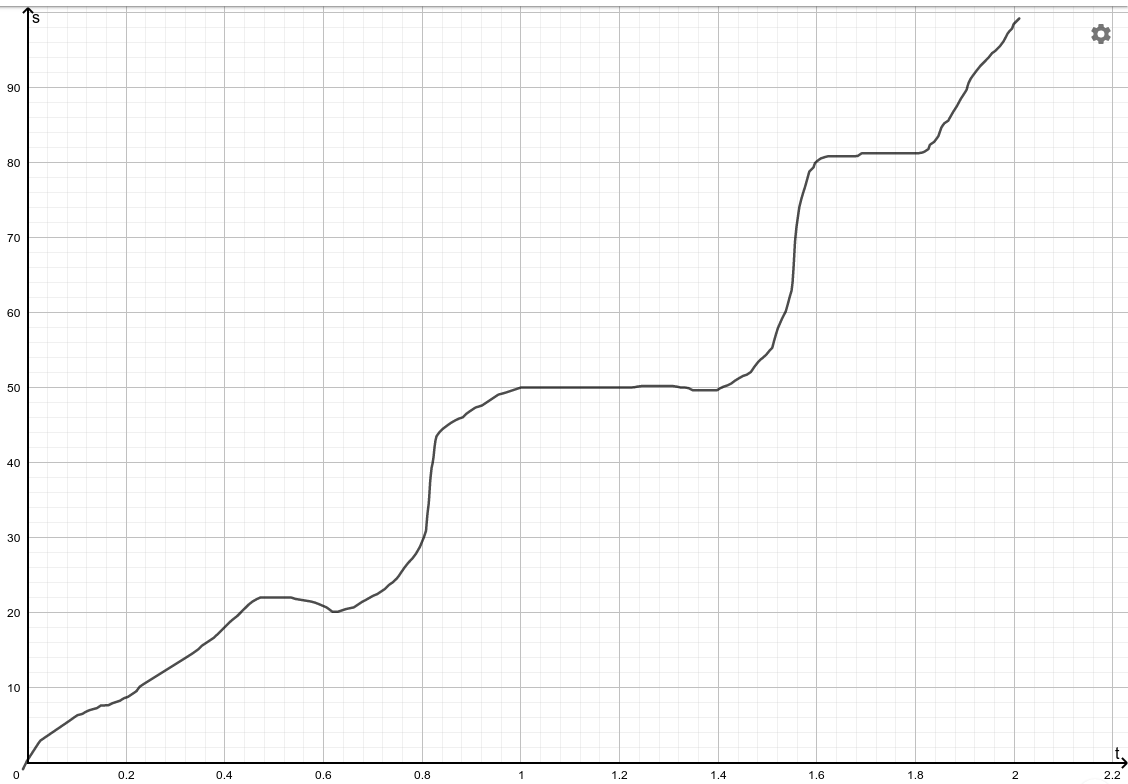
\includegraphics[width=0.5\linewidth]{displacement-as-a-function-of-time.png}
                            \caption{Displacement as a Function of Time}
                            \label{fig: displacement-as-a-function-of-time}
                        \end{figure}
                Even though we have transitioned into the ``continuous", the \emph{average speed} does not change because its definition is still the same -- a ratio of the total displacement to the total time. No matter what happens between the two points to the line representing the journey, the average velocity and average speed are the same as long as the points representing the start and finish are the same. Thus, if a particle moves from a point $(\vect{s_1}, t_1)$ on this 2-D plane to another point $(\vect{s_2}, t_2)$, then the average speed
                $$
                    v_{av} = \frac{|\vect{s_2}-\vect{s_1}|}{t_2-t_1}
                $$
                
                And, since velocity is a vector, the \emph{average velocity}
                $$
                    \vect{v_{av}} = \frac{\vect{s_2}-\vect{s_1}}{t_2-t_1}
                $$

                This is shown in Figure \ref{fig: average-speed-depends-only-on-end-points}. 
                        \begin{figure}[h!]
                            \centering
                            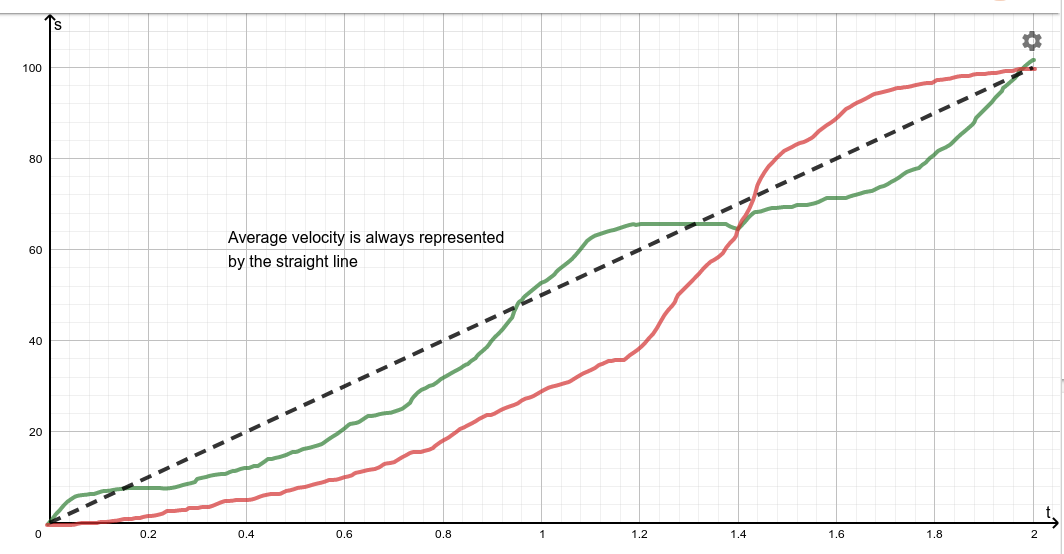
\includegraphics[width=0.6\linewidth]{average-velocity-only-depends-on-end-points.png}
                            \caption{Average Speed Depends Only on End-points}
                            \label{fig: average-speed-depends-only-on-end-points}
                        \end{figure}
                
                Note that the direction of the average velocity vector, $\vect{v_{av}}$, is the same as the direction of the vector that represents the difference of two vectors, $\vect{s_1}$ and $\vect{s_2}$, and the average speed, $v_{av}$, represents the \emph{magnitude} of the velocity vector.

                Since the average velocity only depends on end points, it does not give us any idea about how fast the particle is moving at an arbitrary point between the start and the finish. It is clear, looking at a lines in Figure \ref{fig: displacement-as-a-function-of-time} and Figure \ref{fig: average-speed-depends-only-on-end-points}, that at some \emph{points in time} the particle appears to be moving much faster than at some other points in time. This very idea of velocity at precise \emph{points in time} or \emph{instants} is interesting and it is called the \emph{instantaneous velocity}.
        \end{enumerate}
    \item Instantaneous Velocity
        \begin{enumerate}
            \item The physicist Richard P. Feynman used to tell a story:

                A lady is caught for speeding \emph{at} 60 miles per hour. She says to the police officer, ``That's impossible, sir, \emph{I have been traveling for only seven minutes}.''

            \item 
        \end{enumerate}

\end{enumerate}

\chapter{Accelerated Motion} \label{ch: 3-accelerated-motion}
\chapter{Force and Equilibrium} \label{ch: 4-force-equilibrium}
\chapter{Various Forces of Nature} \label{ch: 5-forces-of-nature}
\chapter{Force, Inertia, and Motion} \label{ch: 6-force-inertia-motion}
\part{Classical Mechanics at Work}
\chapter{Using Newton's Law} \label{ch: 7-newtons-law}
\chapter{Universal Gravitation}\label{ch: 8-universal-gravitation}
\chapter{Collisions and Conservation Laws} \label{ch: 9-collisions}
\chapter[Energy Conservation in Dynamics]{Energy Conservation in Dynamics; Vibrational Motions}\label{ch: 10-energy-conservation}
\chaptermark{Energy Conservation}








\appendix
\chapter{History of Zeno's Paradoxes on Motion}
\label{zeno}
\begin{enumerate}
    \item Zeno's arguments have come to us via Plato, Aristotle, and Simplicius. And, of course, these arguments are understood from the translations of the Greek classics.
    \item The four arguments of Zeno \emph{against the notion of motion}:
        \begin{enumerate}
            \item \textbf{Dichotomy\footnote{Contrast or difference between two opposing things or ideas}}: You cannot traverse infinite \emph{space} (thought of as a collection of an infinite number of \emph{points}) in finite amount of \emph{time}. This is akin to the reasoning that a rubber ball with a coefficient of restitution, say, 0.5 can never come to a standstill because it could not have made infinite number of bounces in a finite amount of time, if, indeed, it does come to a standstill.
            \item \textbf{Achilles}: Achilles will never be able to beat the tortoise if tortoise has a head start even if Achilles is \emph{faster} of the two.
            \item \textbf{Arrow}:
            \item \textbf{Stade}:
        \end{enumerate}
\end{enumerate}


\begin{thebibliography}{00}
    \bibitem{apf} A. P. French. Newtonian Mechanics. M.I.T. Introductory Physics Series. Thomas Nelson and Sons Ltd. Available to borrow digitally at \href{http://archive.org}{archive.org}.
    \bibitem{pf} \href{https://physicsforums.com}{The Physics Forums}.
    \bibitem{iaam} Paul Richard Halmos. I Want to be a Mathematician -- An Automathography. Springer. 1st Edition, 1985.
    \bibitem{cajori-zeno} Florian Cajori. The History of Zeno's Arguments on Motion. The American Mathematical Monthly. 1915.
    \bibitem{copernicus} Nicolaus Copernicus. \textit{De Revolutionibus orbium colelestium}. 1543. The \href{https://en.wikipedia.org/wiki/Nicolaus_Copernicus#The_book}{Wikipedia page}.
    \bibitem{neptune} Siddarth Bhatnagar and Jayant Murthy. Game of Orbits: A Gaming Approach to Neptune's Discovery. July 31, 2018. On \href{https://arxiv.org/pdf/1807.11280.pdf}{Arxiv}.
    \bibitem{polya-guessing} George P{\'o}lya. Let's Teach Guessing. The Mathematical Association of America Video. \href{https://www.youtube.com/watch?v=h0gbw-Ur_do}{YouTube video}.
    \bibitem{newton-bt} Isaac Newton's \href{https://en.wikipedia.org/wiki/Binomial_theorem#Newton's_generalized_binomial_theorem}{Generalization} of the Binomial Theorem (also known as the Binomial Series). 
    \bibitem{cosm} Ethan D. Bolker and Maura B. Mast. Common Sense Mathematics: Second Edition. MAA Press. \href{https://bookstore.ams.org/text-63}{Volume 63; 2021}.
    \bibitem{malthus} Thomas Robert Malthus. \href{https://en.wikipedia.org/wiki/An_Essay_on_the_Principle_of_Population}{An Essay on the Principle of Population}. 1798.
    \bibitem{davidson} Martin Davidson (and Cameron Dinwoodie). Elements of Mathematical Astronomy (Third Edition). Hutchinson Scientific and Technical. 1962.
    \bibitem{universe-today} Matt Williams. What is Asteroid Belt?. \href{https://www.universetoday.com/32856/asteroid-belt/}{Universe Today}. 23 August 2015.
    \bibitem{desmos} \href{https://www.desmos.com}{Desmos}. 
    \bibitem{Neptune-data} Miner, E. D.. "\href{https://www.britannica.com/place/Neptune-planet}{Neptune}". Encyclopedia Britannica, March 2, 2021. 
    \bibitem{oerter} Robert Oerter. The Theory of Almost Everything -- The Standard Model, the Unsung Triumph of Modern Physics. Penguin USA. September 2006.
    \bibitem{the-standard-model} \href{https://en.wikipedia.org/wiki/Standard_Model}{The Standard Model}.
    \bibitem{principia} Issac Newton. English translation by Andrew Mott. Newton's Principia: the Mathematical Principles of Natural Philosophy. University of California Libraries. 1846. \href{https://archive.org/details/newtonspmathema00newtrich/page/n27/mode/2up}{On Archive.org}.
    \bibitem{adewole} Adewole, A I A. Newton On Absolute Space: A Commentary. October 2001. \href{https://cds.cern.ch/record/523046}{CERN Document Server}.
    \bibitem{pssc-for} Frames of Reference. Physical Science Study Committee. 1960. \href{https://archive.org/details/FramesOfReference_201407}{Black-and-white video}.
    \bibitem{polar} \href{https://en.wikipedia.org/wiki/Spherical_coordinate_system}{The Spherical Coordinate System}.
    \bibitem{vector-wikipedia} \href{https://en.wikipedia.org/wiki/Vector_(mathematics_and_physics)}{Vector (Mathematics and Physics}.
    \bibitem{resolution-q-phy-fo}  \href{https://www.physicsforums.com/threads/axes-of-the-2-d-coordinate-system-used-in-vector-resolution.1001481/}{Axes of the 2-d coordinate system used in vector resolution}.
    \bibitem{nbs-time-freq} Time and Frequency: Theory and Fundamentals. Byron E. Blair, Editor. National Bureau of Standards Monograph 140. May 1974.
    \bibitem{sundials-atomic} From Sundials to Atomic Clocks: Understanding Time and Frequency. James Jespersen and Jane Fitz-Randolph. NBS Monograph 155. March 1999.
    \bibitem{nist-revised-si} Redefining the World's Measurement System. On the WWW at \href{https://www.nist.gov/si-redefinition/turning-point-humanity-redefining-worlds-measurement-system}{the NIST website}.
    \bibitem{voices-of-time} J. T. Fraser (ed.). The Voices of Time. George Braziller, New York. 1966.
    \bibitem{pssc-physics} Uri Haber-Schaim, Judson B. Cross, John H. Dodge, James A. Walter. PSSC Physics Third Edition 1971. D. C. Heath and Company Lexington, Massachusetts.
    \bibitem{pim} Eric M. Rogers. Physics for the Inquiring Mind -- the Methods, Nature, and Philosophy of Physical Science. Princeton University Press. Fourth Printing 1962.
    \bibitem{tpim} Eric M. Rogers. Teaching Physics for the Inquiring Mind -- an informal commentary on physics teaching in general and the teaching of science to non-scientists in particular. Princeton University Press. 1962. 
    \bibitem{intro-to-phy-mass-length-time} Norman Feather. An Introduction to the Physics of Mass, Length, and Time. Edinburgh University Press. 1959.
    \bibitem{stf} G. M. Clemence. Standards of Time and Frequency. Science, Vol. 123 Issue 3197 (April 06, 1956).
    \bibitem{stf21} S. A. Diddams, J. C. Bergquist, S. R. Jefferts, C. W. Oates. Standards of Time and Frequency at the Outset of the 21st Century. Science, Vol. 306 Issue 5700 (19 Nov 2004).
    \bibitem{nature-of-time} Thomas Gold and D. L. Schumacher. The Nature of Time. Cornell University Press. Ithaca, N. Y. 1967.
    \bibitem{time-and-physical-world} Richard Schlegel. Time and Physical World. Dover, New York. 1968.
\end{thebibliography}
\end{document}
